\documentclass[
book,
%a4paper,					% alle weiteren Papierformat einstellbar
%landscape,					% Querformat
11pt,						% Schriftgr�ߟe (12pt, 11pt (Standard))
BCOR0.8cm,					% Bindekorrektur, bspw. 1 cm
%DIVcalc,					% f�hrt die Satzspiegelberechnung neu aus
twoside,					% einseitiges Layout
%twocolumn,					% zweispaltiger Satz
%openany,					% Kapitel k�nnen auch auf linken Seiten beginnen
%halfparskip*,				% Absatzformatierung s. scrguide 3.1
%notitlepage,				% in-page-Titel, keine eigene Titelseite
%chapterprefix,				% vor Kapitel�berschrift wird "Kapitel Nummer" gesetzt
%appendixprefix,			% Anhang wird "Anhang" vor die ܜberschrift gesetzt 
%normalheadings,			% ܜberschriften etwas kleiner (smallheadings)
%idxtotoc,					% Index im Inhaltsverzeichnis
%liststotoc,				% Abb.- und Tab.verzeichnis im Inhalt
%bibtotoc,					% Literaturverzeichnis im Inhalt
bibliography=totoc,
%leqno,						% Nummerierung von Gleichungen links
%fleqn,						% Ausgabe von Gleichungen linksb�ndig
%draft						% �berlangen Zeilen in Ausgabe gekennzeichnet
]{scrreprt}

% ============================ Packages ============================ 

%\usepackage[inner=3.0cm,outer=2.5cm,top=1.5cm,bottom=1.5cm,includeheadfoot]{geometry}
									% Einstellungen der Seitenr�nder
\usepackage[includeheadfoot]{geometry}
\usepackage[T1]{fontenc}				% neue Rechtschreibung
\usepackage[latin1]{inputenc}		         % Umlaute erm�glichen
\usepackage[german, english]{babel}
\usepackage{fancyhdr}				% f�r Kopf- und Fuߟzeile
\usepackage[hyperref]{xcolor}		
\definecolor{MyBlue}{RGB}{50,79,132}		% f�r Kopf- und Fu�zeile
\usepackage[colorlinks, citecolor=MyBlue, linktocpage, linkcolor=MyBlue]{hyperref}
\usepackage{color}					% Farbe
\usepackage[pdftex]{graphicx}
\usepackage{float}
\usepackage{listings}				% Programm-Code
\usepackage{longtable}				% Tabellen �ber mehrere Seiten
\usepackage{siunitx}				% Einheiten nach SI-Norm
\usepackage{listings}                                    % Verwendung von Matlab-Code
\usepackage{amsmath}
\usepackage{amssymb}
\usepackage{mathtools}
\usepackage[tight]{subfigure}
\usepackage{empheq}
\usepackage{overcite}
\usepackage{url}
\usepackage{framed}
\usepackage{pdfpages}
\usepackage[compact]{titlesec}
% ============================ Kopf- und Fu�zeile ==========================

\pagestyle{fancy}
\fancyhf{}

\fancyhead[CO,CE]{\scshape\leftmark}	% Kopfzeile links [L], mitte [C], rechts [R]
\fancyfoot[RO,LE]{\thepage}				% Fu�zeile
\renewcommand{\headrulewidth}{0.5pt}	% Linie oben
\renewcommand{\footrulewidth}{0pt}		% Linie unten
\pagenumbering{roman}

%============================ new Definitions ============================
%============================ Befehlsdefinitionen============================

\newcommand{\beq}{\begin{eqnarray}}		% Abk�rzung f�r nummerierte Gleichungen
\newcommand{\eeq}{\end{eqnarray}}		% Ab�rzung f�r nummerierte Gleichungen
\newcommand{\nn}{\nonumber}				% Abk�rzung f�r nummernlose Gleichung
\newcommand{\dm}{\mathrm{d}}			% Abk�rzung f�r Differential/Integral d
\newcommand{\del}{\partial}				% Partielle Ableitung
\newcommand{\bal}{\begin{aligned}}
\newcommand{\eal}{\end{aligned}}
\newcommand*\widefbox[1]{\fbox{\hspace{2em}#1\hspace{2em}}}
\renewcommand\citeform[1]{[#1]}


\setcounter{secnumdepth}{3}
%\setlength{\subfigtopskip}{cm}
% ==================  New Chapter/Section Definition  =====================

%\titleformat{?command?}[?shape?]{?format?}{?label?}{?sep?}{?before-code?}[?after-code?]
\titlespacing{\chapter}{0pt}{0pt}{20pt}
\titleformat{\chapter}[display]{\bfseries\Large \color{MyBlue}}{\filleft \fontsize{50}{20} \selectfont \thechapter}{.5em}{\titlerule \vspace{2ex}}[\vspace{2ex} \titlerule]
\titleformat{\section}
  {\normalfont \filcenter \large\bfseries \color{MyBlue}}{\thesection}{1em}{}
%========================= Document ==============================
\include{titlePageDefinition}
% =============================Titelseite ==================================

\begin{document}

\pagenumbering{roman}

  \LMUTitle
      {FDTD Simulation von Elektronenstreuung an einer elektromagnetischen Welle}               % deutscher Titel der Arbeit
      {FDTD Simulation of electron scattering in an electromagnetic wave}			% english title
      {David Symhoven}                       % Vor- und Nachname des Autors
      {Witten}                             % Geburtsort des Autors
      {Computational \& Plasma Physics}                         % Name des Lehrstuhls
      {M�nchen 2017}                          % Ort und Jahr der Erstellung
      {18.07.2017}                            % Tag der Abgabe
      {Prof.Dr.Hartmut Ruhl}                          % Name des Erstgutachters
      {Zweitgutachter}                         % Name des Zweitgutachters



%======================== EINLEITUNG ========================
%===========================================================
\chapter*{Introduction}
Now it's going loose ...  \cite{Allen}\\
What is the goal of this thesis?\\
What is Plasma, and where is it used ? \\
Summary of all chapters\\
%Literatur Fennel / King

%================================= SYMBOLE UND KONTANTEN ================
\chapter*{Symbols and Constants}


\begin{tabular}{lll}
%Plank'sches Wirkungsquantum  	& \qquad h  			&  \qquad 6.62606957(29) $\cdot 10^{-34}~\si{\joule\second}$ \\ 
%Plank'sches Wirkungsquantum	  	&  \qquad $\hbar$  		&  \qquad1.054571726(47) $\cdot 10^{-34}~\si{\joule\second}$ \\
%Boltzmann - Konstante			& \qquad $k_{B}$ 		& \qquad  1.3806488(13) $\cdot 10^{-23}~\si{\joule\per\kelvin}$\\
%Avogadro - Konstante			& \qquad $N_A$ 		& \qquad 6.02214129(27) $\cdot 10 ^{23}~\si{\per\mole}$\\
Vacuum permittivity				& \qquad $\epsilon_0$	& \qquad 8.85418781762 $\cdot 10 ^{-12}~\si{\ampere\second\per\volt\per\meter}$\\
Vacuum permeability				& \qquad $\mu_0$		& \qquad 2566370614 $\cdot 10 ^{-6}~\si{\newton\per\square\ampere}$\\
%atomare Masseneinheit			& \qquad u 			& \qquad 1.660538921(73) $\cdot 10^{-27} ~\si{\kilogram}$\\
%Elektronenvolt					& \qquad eV			& \qquad 1.602176565(35) $\cdot 10^{-19}~\si{\joule}$\\
\noalign{\vskip 5mm}
Electrical flux density				& \qquad $\vec{D}$		& \qquad $[\si{\ampere\second\per\square\meter}]$\\
Magnetic flux density				& \qquad $\vec{B}$		& \qquad $[\si{\tesla}]$\\
Magnetic field strength			& \qquad $\vec{H}$		& \qquad $[\si{\ampere\per\meter}]$\\
Electric field stength				& \qquad $\vec{E}$		& \qquad $[\si{\volt\per\meter}]$\\
%1 Angstr�m 					& \qquad $\si{\angstrom}$  	& \qquad  $10^{-10}~\si{\meter}$ \\
%1 Nanosekunde 				& \qquad $\si{\nano\second}$  	& \qquad $10^{-9}~\si{\second}$ \\
%1 Pikosekunde 					& \qquad $\si{\pico\second}$ 	& \qquad $10^{-12}~\si{\second}$ \\
%1 Femtosekunde				& \qquad $\si{\femto\second}$ 	& \qquad $10^{-15}~\si{\second}$ \\

\noalign{\vskip 5mm}

%Ort							& \qquad $\vec{r}$			& \qquad $[\si{\meter}]$\\
%Geschwindigkeit				& \qquad $\vec{v}$ 			& \qquad $[\si{\meter\per\second}]$ \\
%Beschleunigung				& \qquad $\vec{a}$ 			& \qquad $[\si{\meter\per\square\second}]$ \\ 
%Impuls						& \qquad $\vec{p}$			& \qquad $[\si{\kilogram\meter\per\second}]$ \\
%Kraft							& \qquad $\vec{F}$ 			& \qquad $[\si{\newton}]$ \\
%Masse						& \qquad m 				& \qquad $[\si{\kilogram}]$ \\
%Energie						& \qquad E 				& \qquad $[\si{\joule}]$ \\
%Temperatur					& \qquad T				& \qquad $[\si{\kelvin}]$ \\
%Druck						& \qquad p 				& \qquad $[\si{\newton\per\square\meter}]$ \\	
%Entropie						& \qquad S				& \qquad $[\si{\joule\per\kelvin}]$ \\
%Potential						& \qquad V				& \qquad \text{nicht eindeutig} \\
%chemisches Potential			& \qquad $\mu$			& \qquad \text{nicht eindeutig} \\
%Zeit 							& \qquad t 				& \qquad $[\si{\second}]$\\
%diskretisierte Zeit				& \qquad $\Delta t$			& \qquad $[\si{\second}]$\\
%Frequenz						& \qquad $\omega$			& \qquad $[\si{\per\second}]$\\
%Gesamtteilchenanzahl			& \qquad N				& \\
%Anzahl der Freiheitsgerade		& \qquad $f$				& \\
%\noalign{\vskip 5mm}

Nabla - Operator				& \qquad $\nabla$			& \qquad  $\left( \frac{\del }{\del r_1}, \ldots, \frac{\del }{\del r_n}\right)$ \\
\noalign{\vskip 2mm}
Laplace - Operator				& \qquad $\Delta$			& \qquad  $\sum_{i=1}^{n} \frac{\del^2}{\del r_i^2}$\\
d'Alembert - Operator			& \qquad $\hat\square$		& \qquad $\Delta- \frac{1}{c^2}\frac{\del^2}{\del t^2}$\\
%\noalign{\vskip 2mm}
%Hamilton - Operator				& \qquad $\mathcal{H}$		& \qquad $\mathcal{H} = -\frac{\hbar^2}{2m}\Delta + V(\vec{r})$ \\		
%\noalign{\vskip 2mm}
%Lagrange - Funktion				& \qquad $\mathcal{L}$		& \qquad $\mathcal{L} = T - V$ \\

\end{tabular}


%================================= Inhaltsverzeichnis ==========================
\tableofcontents

%============================ Beginn Textseiten ================================
\pagenumbering{arabic}



%================================= Bildvorlage ====================================

%Code f�r Bildumgebung
%\begin{figure}[H]
%	\centering
%		\includegraphics[width=0.50\textwidth]{Destruktive_Interferenz.jpg} %Bild 1
%	\caption[Destruktive Interferenz]{Destruktive Interferenz \cite{[Wiki12]}}
%	\label{fig:Interferenzfilterr}
%\end{figure}
%\noindent

%===========================================================================

%======================== FUNDAMENTALS ========================
%===========================================================
\part{Fundamentals}
\noindent
In this first part we present the theoretical basics this thesis is built upon. We start with the foundation of electromagnetism - the Maxwell Equations - followed by the corresponding potential equations. Introducing Lorentz-Gauge will lead us to the inhomogeneous wave equation, which we will solve using Greens-function approach. This will lead us to the Li�nard-Wiechert potentials, which are key in this thesis. Lastly we discuss both the non relativistic and relativistic phenomenon of energy radiation, where we restrict ourselves to the simple case where a particle is accelerated parallel to its direction of motion.
%======================== Electromagnetic radiation ========================
%===========================================================
\chapter{Electromagnetic radiation}
\section{Maxwell-Equations}
The Maxwell equations are the foundation of the classical electromagnetism and describe how the electric field strength $\vec{E} \in \mathbb{R}^3$ and the magnetic field strength $\vec{H} \in \mathbb{R}^3$ are generated by charges and currents respectively and how they evolve over time in space in presence of one another. In presence of matter however, the interaction of the fields with the material need to be taken into account. The effect of microscopic dipols, formed by bound charge carriers, are summarized in macroscopic entities called Polarisation $\vec{P} \in \mathbb{R}^3$ and Magnetization $\vec{M} \in \mathbb{R}^3$. These dipols align in the external field such that the resulting electric and magnetic field are described by
\beq
\bal
\label{eqn: materialEquationsFull}
\vec{D} &\coloneqq \epsilon_0 \vec{E} + \vec{P}\\
\vec{H} &\coloneqq \frac{1}{\mu_0} \vec{B} - \vec{M},
\eal
\eeq
where $\mu_0$ and $\epsilon_0$ are the vacuum permeability and permittivity respectively. The macroscopic Maxwell Equations than read
\beq
\label{eqn: maxwellEq}
\label{eqn: maxwell1}
\vec{\nabla} \vec{B} &=& 0\\
\label{eqn: maxwell2}
\vec{\nabla} \vec{D} &=& \rho \\
\label{eqn: maxwell3}
\vec{\nabla} \times \vec{E} &=& - \frac{\del \vec{B}}{\del t}\\
\label{eqn: maxwell4}
\vec{\nabla} \times \vec{H} &=& \frac{\del \vec{D}}{\del t} + \vec{j},
\eeq
where $\rho$ denotes the charge density of the electric source and $\vec{j}$ the electric current density. \\
In the case of vacuum, the material equations \eqref{eqn: materialEquationsFull} reduce to 
\beq
\bal
\label{eqn: materialEquations}
\vec{D} &= \epsilon_0 \vec{E}\\
\vec{H} &= \frac{1}{\mu_0} \vec{B}.
\eal
\eeq

%======================== Colomb and Lorentz Gauge ========================
\section{Colomb and Lorentz Gauge}
In the following section we consider the Maxwell Equations in vacuum.\\
The electric and magnetic fields can also be described by a scalar and a vector potential respectively. From \eqref{eqn: maxwell1} we can conclude that 
\beq
\label{eqn: vecA}
\exists \vec{A} \in \mathbb{R}^3 \colon \vec{B} = \vec{\nabla} \times \vec{A},
\eeq
where $\vec{A}$ is called the vector potential. Plugging in \eqref{eqn: vecA} into \eqref{eqn: maxwell3} yields
\beq
\label{eqn: varphi}
\vec{\nabla} \times \left( \vec{E} + \frac{\del \vec{A}}{\del t}\right) &=& 0.\nn \\
\Rightarrow \exists \varphi \in \mathbb{R} \colon \vec{E} + \frac{\del \vec{A}}{\del t} &=& -\vec{\nabla} \varphi.
\eeq
$\varphi$ is called scalar potential. Plugging in \eqref{eqn: varphi} into \eqref{eqn: maxwell2} and also \eqref{eqn: vecA} and \eqref{eqn: varphi} into \eqref{eqn: maxwell4} gives the potential equations
\beq
\bal
\label{eqn: potentialEquations}
- \Delta \varphi - \vec{\nabla} \left(\frac{\del \vec{A}}{\del t}\right) &= \frac{\rho}{\epsilon_0} \\
\underbrace{\left(\Delta- \frac{1}{c^2}\frac{\del^2}{\del t^2}\right)}_{\coloneqq \hat\square} \vec{A} - \vec{\nabla} \left(\vec{\nabla} \vec{A} + \frac{1}{c^2}\frac{\del \varphi}{\del t}\right) &= -\mu_0\vec{j},
\eal
\eeq
where we used the \textit{Gra�mann Identity}: $\vec{\nabla} \times (\vec{\nabla} \times \vec{A}) = \vec{\nabla}(\vec{\nabla}\vec{A}) - \Delta \vec{A}$.\\
The description of the fields by the aforementioned potentials $\varphi$ and $\vec{A}$ are not unique. This is called gauge freedom. The potentials can be specifically adjusted to the problem at hand. The gauge transformations look like
\beq
\bal
\vec{A} \mapsto \vec{A}' = \vec{A} + \vec{\nabla} \psi\\
\varphi \mapsto \varphi' = \varphi - \frac{\del \psi}{\del t},
\eal
\eeq
where $\psi \colon \mathbb{R}^3 \times \mathbb{R} \mapsto \mathbb{R}$. In appendix \ref{appendix: Gauge Transformations} we show, that $\psi$ does indeed not change the physics.\\
\newline
If we choose $\psi$ such that 
\beq
\label{eqn: LaurentzGauge}
\vec{\nabla} \vec{A} + \frac{1}{c^2}\frac{\del \varphi}{\del t} = 0,
\eeq
then we call it a \textit{Lorentz Gauge} and the potential Equations \eqref{eqn: potentialEquations} decouple into two separate wave equations
\beq
\label{eqn: waveEquations}
\bal
\hat\square \varphi &= -\frac{\rho}{\epsilon_0} \\
\hat\square \vec{A} &= -\mu_0\vec{j}.
\eal
\eeq

%======================== Li�nard-Wiechert Potentials ========================
\section{Li�nard-Wiechert Potentials}
\label{sec: lw-potentials}
\subsection{Solution of inhomogeneous wave equation}
The \textit{Li�nard-Wiechert} Potentials are the solution of \eqref{eqn: waveEquations}. Following \cite{Nolting} we solve the general case
\beq
\label{eqn: generalWaveEquation}
\hat\square \psi(\vec{r}, t) = f(\vec{r},t),
\eeq
where $\psi, f: \mathbb{R}^3 \times \mathbb{R} \mapsto \mathbb{R}$. $f$ is called source function and will be specified later. \eqref{eqn: generalWaveEquation} is a linear inhomgeneous partial differential equation. Those kind of equations are solved with the \textit{Green's function} approach. If we can find the Green's function G fulfilling
\beq
\label{eqn: Greens function}
\hat\square G(\vec{r} - \vec{r}~', t - t') = - \delta(\vec{r} - \vec{r}~')\delta(t - t'),
\eeq
then we can calculate the solution of \eqref{eqn: generalWaveEquation} via
\beq
\label{eqn: WaveEquationSolution}
\psi(\vec{r}, t) = \int \int G(\vec{r} - \vec{r}', t - t') f(\vec{r},t) \dm t' ~\dm \vec{r}~'.
\eeq
To find G we use the following Fourier - Transformations 
\beq
\label{eqn: FourierTransforms}
\bal
G(\vec{r} - \vec{r}~', t - t') &= \frac{1}{4\pi^2} \int \int G(\vec{k}, \omega) \exp(i\vec{k}(\vec{r} - \vec{r}~'))\exp(-i\omega(t - t')) \dm \omega~\dm \vec{k}, \\
\delta(\vec{r} - \vec{r}~') &= \frac{1}{4\pi^2} \int \exp(i\vec{k}(\vec{r} - \vec{r}~')) \dm \vec{k}, \\
\delta(t - t') &= \frac{1}{4\pi^2} \int \exp(-i\omega(t - t')) \dm \omega.
\eal
\eeq
Plugging in \eqref{eqn: FourierTransforms} into \eqref{eqn: Greens function} yields
\beq
\int \int \exp(i\vec{k}(\vec{r} - \vec{r}~'))\exp(-i\omega(t - t')) \left[ G(\vec{k}, \omega) \left( -k^2 + \frac{\omega^2}{c^2}\right) + \frac{1}{4\pi^2} \right] = 0, \nn
\eeq
which leaves us with
\beq
G(\vec{k}, \omega) = \frac{1}{4\pi^2} \frac{1}{k^2 - \frac{\omega^2}{c^2}}. \nn
\eeq
Using residue theorem we find the Fourier Back Transform of G to be
\beq
\label{eqn: Gret}
G_{ret}(\vec{r} - \vec{r}~', t - t') = \frac{\delta(t' - t_{ret})}{4\pi |\vec{r} - \vec{r}~'|},
\eeq 
where 
\beq
t_{ret} \coloneqq t - \frac{|\vec{r} - \vec{r}~'|}{c} 
\eeq
is the retarded time. We also call $G_{ret}$ the \textit{retarded Green's function} in contrast to the \textit{advanced Green's function} $G_{av}$ with the advanced time
\beq
t_{av} \coloneqq t + \frac{|\vec{r} - \vec{r}~'|}{c}.
\eeq
The latter does not fulfill the causal principle of physics. We expect the reason for a change in our signal at $\vec{r}$ at time t, due to a perturbation, to be in the past, not the future. Because $t_{ret} < t$ the retarded Green's function is the one to work with. Plugging in \eqref{eqn: Gret} into \eqref{eqn: WaveEquationSolution} yields
\beq
\psi(\vec{r}, t) = \frac{1}{4\pi}\int \frac{f(\vec{r}~', t_{ret})}{|\vec{r} - \vec{r}~'|} \dm \vec{r}~',
\eeq
which finally leads to the retarded potential equations
\beq
\varphi(\vec{r},t) &=& \frac{1}{4\pi \epsilon_0} \int \frac{\rho(\vec{r}~', t_{ret})}{|\vec{r} - \vec{r}~'|} \dm \vec{r}~',\\
\vec{A}(\vec{r},t) &=& \frac{\mu_0}{4\pi} \int \frac{\vec{j}(\vec{r}~', t_{ret})}{|\vec{r} - \vec{r}~'|} \dm \vec{r}~'.
\eeq
Lastly we show in Appendix \ref{appendix: Retarded Potential Equations Fulfill Laurentz Gauge} that they indeed fulfill the Laurentz Gauge \eqref{eqn: LaurentzGauge}.

\subsection{Special Case: Moving point charge}
Now we want to discuss the special case of a particle with charge q, moving along the trajectory $\vec{r}_p$ with velocity $\vec{v} \coloneqq \dot{\vec{r}}_p$, where the dot donates the time derivative. As mentioned before, we now define the source functions for our problem at hand. For the charge density we have
\beq
\rho(\vec{r}, t) = q\delta(\vec{r} - \vec{r}_p(t))
\eeq
and for the current density
\beq
\vec{j}(\vec{r}, t) = q\vec{v}\delta(\vec{r} - \vec{r}_p(t)).
\eeq
Identifying 
\beq
\bal
\psi(\vec{r},t) &= \varphi(\vec{r},t)~\text{and}~f(\vec{r}~',t') = \frac{\rho(\vec{r}~',t')}{\epsilon_0}, \nn\\
\vec{\psi}(\vec{r},t) &= \vec{A}(\vec{r},t)~\text{and}~\vec{f}(\vec{r}~',t') = \mu_0\vec{j}(\vec{r}~',t')
\eal
\eeq
and using \eqref{eqn: WaveEquationSolution} with \eqref{eqn: Gret} yields after integrating over $\vec{r}~'$
\beq
\bal
\varphi(\vec{r},t) &= \frac{1}{4\pi \epsilon_0} \int \frac{\delta\left(\frac{ |\vec{r} - \vec{r}_p|}{c} - t + t'\right)}{|\vec{r} - \vec{r}_p|} \dm t',\\
\vec{A}(\vec{r},t) &= \frac{q \mu_0}{4\pi} \int \vec{v}(t')\frac{\delta\left(\frac{ |\vec{r} - \vec{r}_p|}{c} - t + t'\right)}{|\vec{r} - \vec{r}_p|} \dm t'.
\eal
\eeq
For the $t'$ - integration we need the following property of the $\delta$ - distribution
\beq
\delta\left[g(t')\right] = \sum_{i = 1}^{n} \frac{\delta(t' - t_i)}{\left| \left( \frac{\dm g}{\dm t'}\right)\Bigr |_{t' = t_i} \right|},
\eeq
where 
\beq
\label{eqn: gDefinition}
g(t') \coloneqq \frac{ |\vec{r} - \vec{r}_p|}{c} - t + t'
\eeq
 and $t_i$ are the roots of $g$. To find the roots of g, let's consider
\beq
\bal
\frac{\dm g}{\dm t'} &= 1+ \frac{1}{c}\frac{\dm}{\dm t'}|\vec{r} - \vec{r}_p|  = 1 - \frac{\vec{v}(t')}{c} \underbrace{ \frac{\vec{r} - \vec{r}_p}{|\vec{r} - \vec{r}_p| }}_{ |\cdot| = 1 }\\
&\Longrightarrow 1 - \frac{\vec{v}(t')}{c} \leq \frac{\dm g}{\dm t'} \leq 1 + \frac{\vec{v}(t')}{c} \\
&\stackrel{v < c}{\Longrightarrow} \frac{\dm g}{\dm t'} > 0,
 \eal
\eeq
which means that g is a monotonically increasing function and therefore has at most one root, which is $t' = t_{ret}$ as can be seen from \eqref{eqn: gDefinition}. In case that g has no roots at all, we can conclude that $\varphi \equiv 0$ and $\vec{A} \equiv 0$.\\
With $t_{ret} \coloneqq t - \frac{|\vec{r} - \vec{r}_p|}{c} $ the integration over $t'$ yields
\beq
\bal
\varphi(\vec{r},t) &= \frac{1}{4\pi \epsilon_0}\frac{q}{|\vec{r} - \vec{r}_p(t_{ret})| - \frac{\vec{v}(t_{ret})}{c}(\vec{r} - \vec{r}_p(t_{ret}))},\\
\vec{A}(\vec{r},t) &= \frac{1 \mu_0}{4\pi} \frac{q\vec{v}(t_{ret})}{|\vec{r} - \vec{r}_p(t_{ret})| - \frac{\vec{v}(t_{ret})}{c}(\vec{r} - \vec{r}_p(t_{ret}))}
\eal
\eeq
which are the \textit{Li�nard-Wiechert} Potentials. Upon defining 
\beq
\bal
\vec{\beta}(t) &\coloneqq \frac{\vec{v}(t)}{c},\\
\vec{R}(\vec{r},t) &\coloneqq \vec{r} - \vec{r}_p(t),\\
\vec{n}(\vec{r},t) &\coloneqq \frac{\vec{R}(\vec{r},t)}{R(\vec{r},t)}
\eal
\eeq
we can rewrite the Li�nard-Wiechert Potentials in a more compact and final form
\beq
\bal
\label{eqn: LWPotentials}
\varphi(\vec{r},t) &= \frac{1}{4\pi \epsilon_0}\frac{q}{(1 - \vec{\beta}(t') \cdot \vec{n}(\vec{r},t')) R(\vec{r},t')}\Biggr |_{t' = t_{ret}},\\
\vec{A}(\vec{r},t) &= \frac{\mu_0}{4\pi} \frac{q\vec{\beta}(t')}{(1 - \vec{\beta}(t') \cdot \vec{n}(\vec{r},t')) R(\vec{r},t')}\Biggr |_{t' = t_{ret}}.
\eal
\eeq
They are the generalization of the Coulomb Potential. With the help of \eqref{eqn: varphi} the electric and magnetic fields can be derived from the \textit{Li�nard-Wiechert} Potentials \eqref{eqn: LWPotentials}. Since this is a quite longish calculation we refer to \cite{Nolting} and just present the final result 
\beq
\label{eqn: Li�nard-Wiechert}
\bal
\vec{E}(\vec{r}, t) &= \frac{q}{4\pi \epsilon_0} \left( \frac{\vec{n}(\vec{r},t') - \vec{\beta}(t)}{ \gamma^2(1 - \vec{\beta}(t) \cdot \vec{n}(\vec{r},t'))^3 R^2(\vec{r},t')} \right. \\
& \left. + \frac{1}{c} \frac{\vec{n}(\vec{r},t') \times (\vec{n}(\vec{r},t') - \vec{\beta}(t)) \times \dot{\vec{\beta}}(t)}{(1 - \vec{\beta}(t) \cdot \vec{n}(\vec{r},t'))^3 R(\vec{r},t')}\right)\Biggr |_{t' = t_{ret}}, \\
\vec{B}(\vec{r}, t) &= \frac{1}{c} \left(\vec{n}(\vec{r},t') \times \vec{E}(\vec{r}, t)\right)\Biggr |_{t' = t_{ret}}.
\eal
\eeq
This is the electric and magnetic field of a moving charged particle. Due to the finite speed of light, the fields need time to travel from their source to the observation point. That means, that the fields at time $t$, were actually produced at a earlier time $t_{ret}$. As can be seen in figure
\ref{fig: Interpolation}, the retarded time is determined by the intersection point of the particle trajectory with the backward lightcone of the observation point.\\

\subsection{Energy emission}
Now we want to discuss the energy flow and emission. Therefore we need to analyze the Poynting Vector
\beq
\label{eqn: PoyntingVector}
\vec{S} = \frac{1}{\mu_0}\vec{E} \times \vec{B} =  \frac{1}{\mu_0 c} \left[ \vec{n}_{ret} E^2  - \left(\vec{n}_{ret} \vec{E}\right) \vec{E}\right],
\eeq
where $\vec{n}_{ret} \coloneqq \vec{n}(\vec{r}, t_{ret})$. Taking a closer look at \eqref{eqn: Li�nard-Wiechert} reveals that both $\vec{E}$ and $\vec{B}$ can be separated into two parts, one of which is not dependent on the particle acceleration 
\beq
\bal
\label{eqn: Ev}
\vec{E}_{(v)}(\vec{r}, t) &= \frac{q}{4\pi \epsilon_0} \frac{1}{ \gamma^2(1 - \vec{\beta}(t') \cdot \vec{n}(\vec{r},t'))^3 R^2(\vec{r},t')} \left(\vec{n}(\vec{r},t') - \vec{\beta}(t')\right)\Biggr|_{t' = t_{ret}}\\
\vec{B}_{(v)}(\vec{r}, t) &= \frac{q}{4\pi \epsilon_0 c} \frac{1}{ \gamma^2(1 - \vec{\beta}(t') \cdot \vec{n}(\vec{r},t'))^3 R^2(\vec{r},t')} \underbrace{\left[\vec{n} \times \left(\vec{n}(\vec{r},t') - \vec{\beta}(t')\right)\right]}_{= \frac{1}{c}\left(\vec{v} \times \vec{n}\right)}\Biggr|_{t' = t_{ret}} 
\eal
\eeq
whilst the other is through $\dot{\vec{\beta}}$
\beq
\bal
\label{eqn: Ea}
\vec{E}_{(a)}(\vec{r}, t) &= \frac{q}{4\pi \epsilon_0c}  \frac{\vec{n}(\vec{r},t') \times \left(\vec{n}(\vec{r},t') - \vec{\beta}(t')\right) \times \dot{\vec{\beta}}(t')}{\left(1 - \vec{\beta}(t') \cdot \vec{n}(\vec{r},t')\right)^3 R(\vec{r},t')}\Biggr |_{t' = t_{ret}}\\
\vec{B}_{(a)}(\vec{r}, t) &= \frac{q}{4\pi \epsilon_0c^2} \frac{\vec{n}(\vec{r},t') \times \left[\vec{n}(\vec{r},t') \times \left(\vec{n}(\vec{r},t') - \vec{\beta}(t')\right) \times \dot{\vec{\beta}}(t')\right]}{\left(1 - \vec{\beta}(t') \cdot \vec{n}(\vec{r},t')\right)^3 R(\vec{r},t')}\Biggr |_{t' = t_{ret}}.
\eal
\eeq
Since $E_{(v)} \propto \frac{1}{R^2}$ whereas $E_{(a)} \propto \frac{1}{R}$, its field contributions will dominate in the far field, i.e. for large distances from the source. Plugging in \eqref{eqn: Li�nard-Wiechert} in \eqref{eqn: PoyntingVector} gives us several terms with different orders of $\frac{1}{R}$, namely
\beq
\bal
\vec{S}_{vv} &\propto \left| \vec{E}_{(v)} \times \vec{B}_{(v)} \right| \propto \frac{1}{R^4},\\
\vec{S}_{va} &\propto \left| \vec{E}_{(v)} \times \vec{B}_{(a)} \right| \propto \frac{1}{R^3},\\
\vec{S}_{aa} &\propto \left| \vec{E}_{(a)} \times \vec{B}_{(a)} \right| \propto \frac{1}{R^2}. \nn
\eal
\eeq
By evaluating the energy flux through an arbitrary surface with differential surface area $\dm\vec{\sigma}$, as illustrated in figure \ref{fig: PoyntingVector},
\begin{figure}[H]
	\centering
		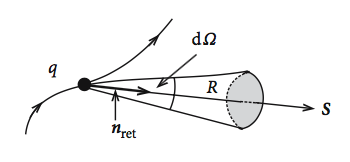
\includegraphics[width=0.50\textwidth]{Pictures/PoyntingVector.png}
	\caption[Illustration of how to calculate the energy emission of a moving particle with charge $q$.]{Illustration of how to calculate the energy emission of a moving particle with charge $q$. \cite{Nolting}}
	\label{fig: PoyntingVector}
\end{figure}
\noindent
we can see, that it will suffice to only consider the $\frac{1}{R^2}$ terms, because the $\frac{1}{R^3}$ or higher terms do not contribute to the energy emission, since
\beq
\oint \vec{S} \dm\vec{\sigma} \rightsquigarrow \oint \frac{1}{R^3} r^2 \dm\Omega \rightsquigarrow \oint \frac{1}{r} \dm\Omega \rightsquigarrow \frac{1}{r} \stackrel{r \rightarrow \infty}{\longrightarrow} 0,
\eeq
where $\dm\Omega \coloneqq \sin(\vartheta)\dm\vartheta\dm\varphi$. That means we can focus on $\eqref{eqn: Ea}$ when calculating $\eqref{eqn: PoyntingVector}$
\beq
\vec{S} =  \frac{1}{\mu_0 c} \frac{q^2}{16\pi^2 \epsilon_0^2 c^2}  \frac{\vec{n}(\vec{r},t') \left[\vec{n}(\vec{r},t') \times \left(\vec{n}(\vec{r},t') - \vec{\beta}(t')\right) \times \dot{\vec{\beta}}(t')\right]^2}{\left(1 - \vec{\beta}(t') \cdot \vec{n}(\vec{r},t')\right)^6 R^2(\vec{r},t')}\Biggr |_{t' = t_{ret}} + \mathcal{O}\left(\frac{1}{R^3}\right).
\eeq
The energy flux has the direction of $\vec{n}_{ret}$, i.e. it flows from the particle position $\vec{r}_p$ at time $t' = t_{ret}$ to the observation point $\vec{r}$. We can also see, that only accelerated particles ($\dot{\vec{\beta}} \neq 0$) loose energy through radiation, which leads to a reduction in kinetic energy. Although an uniformly moving particle produces E and B - fields, it does not loose energy through radiation.\\
\newline
Lastly we want to discuss the radiation power. The emitted energy per time $\dm t$ into the solid angle $\dm \Omega$ is described by
\beq
\frac{\dm W}{\dm \Omega} = \left( \vec{S} \cdot \vec{n}(\vec{r}, t') \right) R^2(\vec{r}, t')\Bigr |_{t' = t_{ret}}.
\eeq
Usually the observed amount of energy per unit time $\dm t$ is not the same as the emitted energy of the particle per unit time $\dm t_{ret}$. To learn more about the emission within the particles system, we want to express our equation in terms of $\dm t_{ret}$, which gives us
\beq
\frac{\dm W}{\dm \Omega} = \left( \vec{S} \cdot \vec{n}(\vec{r}, t') \right) R^2(\vec{r}, t') \left(\frac{\dm t}{\dm t'}\right)\Bigr |_{t' = t_{ret}}.
\eeq
From the definition of $t_{ret} \coloneqq t' - \frac{|\vec{r} - \vec{r}~'|}{c}$ we find
\beq
\left(\frac{\dm t}{\dm t'}\right)\Bigr |_{t' = t_{ret}} = \left(1 + \frac{1}{c} \frac{\dm}{\dm t'} |\vec{r} - \vec{r}_p(t')|\right)\Bigr |_{t' = t_{ret}} = \left(1 - \frac{1}{c} \vec{n}(\vec{r}, t')\vec{v}(t')\right)\Bigr |_{t' = t_{ret}}.
\eeq
Finally we obtain
\beq
\label{eqn: RadiationPower}
\frac{\dm W}{\dm \Omega} =  \frac{q^2}{16\pi^2 \epsilon_0 c}  \frac{ \left[\vec{n}(\vec{r},t') \times \left(\vec{n}(\vec{r},t') - \vec{\beta}(t')\right) \times \dot{\vec{\beta}}(t')\right]^2}{\left(1 - \vec{\beta}(t') \cdot \vec{n}(\vec{r},t')\right)^5} \Biggr |_{t' = t_{ret}}.
\eeq
Now we can discuss two cases. The non relativistic case ($\beta \approx 0$) and the relativistic case ($\beta \approx 1$).\\
\begin{description}
\item[$\beta \approx 0$:] In this case \eqref{eqn: RadiationPower} simplifies to
\beq
\bal
\frac{\dm W}{\dm \Omega} &=  \frac{q^2}{16\pi^2 \epsilon_0 c}   \left[\vec{n}(\vec{r},t') \times \left(\vec{n}(\vec{r},t') \times \dot{\vec{\beta}}(t')\right)\right]^2 \Biggr |_{t' = t_{ret}} \\
&=  \frac{q^2}{16\pi^2 \epsilon_0 c}   \left[\underbrace{\left(\vec{n}(\vec{r},t') \cdot \dot{\vec{\beta}}(t') \right)}_{= \dot{\beta}n\cos(\vartheta)} \vec{n}(\vec{r},t') - \underbrace{\left(\vec{n}(\vec{r},t') \cdot \vec{n}(\vec{r},t')\right)}_{ |\cdot| = 1} \dot{\vec{\beta}}(t')\right]^2 \Biggr |_{t' = t_{ret}} \\
& = \frac{q^2\dot{\beta}^2_{ret}}{16\pi^2 \epsilon_0 c}  \left(\cos^2(\vartheta) - 2\cos^2(\vartheta) + 1\right)\\
&=  \frac{q^2 \dot{\beta}^2_{ret}}{16\pi^2 \epsilon_0 c} \sin^2(\vartheta) \nn,
\eal
\eeq 
where $\vartheta$ is the angle between $\dot{\vec{\beta}}$ and $\vec{n}$. $\beta_{ret}$ means again the evaluation at $t' = t_{ret}$. We conclude, that the direction of maximum radiation is perpendicular to the particles direction of motion, in contrast to
\item[$\beta \approx 1$:] where we will see shortly, that the maximum radiation will be primarily in the direction of motion of the particle. We will restrict ourselves to the simple case, where $\dot{\vec{\beta}} \parallel \vec{\beta}$. Following the same steps as above we obtain
\beq
\frac{\dm W}{\dm \Omega} = \frac{q^2 \dot{\beta}^2_{ret}}{16\pi^2 \epsilon_0 c} \frac{\sin^2(\vartheta)}{\left(1 - \beta(t')\cos(\vartheta)\right)^5}.
\eeq
The get the angle, where the radiation is maximal, we calculate
\beq
\bal
\frac{\dm}{\dm(\cos(\vartheta))} &\left(\frac{\dm W}{\dm \Omega}\right) \stackrel{!}{=} 0 \\
\Longleftrightarrow& -2\cos(\vartheta)\left(1-\beta_{ret}\cos(\vartheta)\right)^5 + 5\beta_{ret}(1-\cos^2(\vartheta))\left(1-\beta_{ret}\cos(\vartheta)\right)^4 \stackrel{!}{=} 0 \\
\Longleftrightarrow& \left(1-\beta_{ret}\cos(\vartheta)\right)^4 \left[-2\cos(\vartheta)\left(1-\beta_{ret}\cos(\vartheta)\right) + 5\beta_{ret}(1-\cos^2(\vartheta))\right] \stackrel{!}{=} 0 \\
\Longrightarrow& -2\cos(\vartheta)\left(1-\beta_{ret}\cos(\vartheta)\right) + 5\beta_{ret}(1-\cos^2(\vartheta)) \stackrel{!}{=} 0 \\
\Longleftrightarrow& \cos^2(\vartheta) + \frac{2}{3\beta_{ret}}\cos(\vartheta) - \frac{5}{3} \stackrel{!}{=} 0\\
\Longrightarrow& \cos(\vartheta)_{max} = \frac{1}{3\beta_{ret}}\left(\sqrt{1+15\beta_{ret}^2} -1\right).\nn
\eal
\eeq
Obviously the angle decreases monotonically with increasing velocity, i.e. increasing $\beta_{ret}$. For $\beta_{ret} = 1$ we get $\cos(\vartheta) = 1$ or equivalently $\vartheta = 0$. In figure \ref{fig: radiationSummary} the results are summarized.
 \begin{figure}[H]
	\centering
		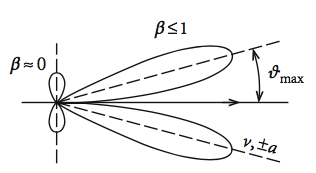
\includegraphics[width=0.50\textwidth]{Pictures/RadiationSummary.png}
	\caption[Radiation characteristics of an moving charged particle]{Radiation characteristics of an moving charged particle. \cite{Nolting}}
	\label{fig: radiationSummary}
\end{figure}
\noindent
\end{description}
 
%======================== NUMERICS ========================
%===========================================================
\part{Numerics}
\noindent
The following section deals with the numeric aspects of this thesis. We explain the underlying equation of motions and their history. After that, we go into several methods with which we can solve differential equations. Over the course of the last decades numerous methods were invented each of which has its own strength and weaknesses. 
Some of them are very easy to implement, which in turn usually leads to unprecise results. Others are quite complicated and sophisticated to implement, but very accurate.
Therefore one should always consider which method is best for the problem and what it is one want to achieve.\\
Following this, we also want to define and calculate the numerical complexity of some chosen algorithms. 

%======================== Integration of equation of motion ========================
%===========================================================
\chapter{Integration of Equation of Motion}
%======================== Equations of Motion ========================
\section{Equations of Motion}
As we know from mechanics the dynamic of a particle is determined by the forces acting on it. In our case there is a force due to electro-magnetic fields. That can be external fields, but also fields due to moving particles, as we explained in section \ref{sec: lw-potentials}.\\
The dynamics of our system is described by the \textit{Lorentz-Newton} equation
\beq
\label{eqn: Lorentz-Newton}
\bal
\frac{\dm x^{\mu}}{\dm \tau} &= u^{\mu}\\
\frac{\dm u^{\mu}}{\dm \tau} &= F^{\mu}_{~\nu}~u^{\nu} + g^{\mu},
\eal
\eeq
which derivation is quite longish, why we want to refer to literature. \\%MISSING: cite
The term $F^{\mu}_{~\nu}$ describes the electromagnetic field strength tensor
\beq
F^{\mu}_{~\nu} = 
\begin{pmatrix}
0 & E_x & E_y & E_z \\
E_x & 0 & B_z & -B_y \\
E_y & -B_z & 0 & B_x \\
E_z & B_y & -B_x & 0
\end{pmatrix}
.
\eeq
The damping term $g^{\mu}$ considers the fact that charged particles radiate fields when they are moving which leads to a loss in their kinetic energy. Within the context of classical electrodynamics Max \textit{Abraham} and Hendrick \textit{Lorentz} discussed radiation damping in their same-named equation first.
In 1938 \textit{Dirac} generalized the equation whilst taking special relativity into account. \\% MISSING: Cites
% MISSING: Details. Historisches. Abraham, Lorentz, Dirac Landau Lifschitz Gleichung usw.
We now want to deal with how to solve the Lorentz-Newton equation \eqref{eqn: Lorentz-Newton} numerically.

%======================== Euler Scheme ========================
\section{Euler-Scheme}
The most simple method is the explicit \textit{Euler}-Method. It's easy to implement but not very accurate, as we shall see later. But before we go into the details of the explicit Euler-Scheme we need to address some prerequisites all following methods will have in common. \\
Starting point will always be a first order system of the kind
\beq
\label{eqn: Euler}
\bal
\frac{\dm x^{\mu}}{\dm \tau} &= u^{\mu}\\
\frac{\dm u^{\mu}}{\dm \tau} &= f^{\mu}(x^{\nu},u^{\nu})\\
x^{\mu}(\tau_0) &= x^{\mu}_0\\
u^{\mu}(\tau_0) &= u^{\mu}_0.
\eal
\eeq
Systems of higher order can always be reduced to a first order system. \\
In order to solve the equation of motion numerically the domain needs to be discretized. Therefore we divide the time interval into N equidistant partial intervals $h$, by defining
\beq
h \coloneqq \Delta \tau = \tau_{i+1} - \tau_i. \nn
\eeq
The idea is to calculate each point along the trajectory $x^{\mu}_i = x^{\mu}(\tau_i)$ iteratively, starting from the initial values $x^{\mu}_0$ and $u^{\mu}_0$.
But to calculate these points all differential operators in  \eqref{eqn: Euler} need to be discretized as well. That is where all methods differ. Each method has its own way to discretize the differential operators.\\
The basis of the Euler-Scheme is a first order Taylor expansion of the integration variable $x^{\mu}$ in $\tau$ around $\tau_i$
\beq
\label{eqn: Taylor}
x^{\mu}(\tau_{i+1}) =  x^{\mu}(\tau_i) + \frac{\dm x^{\mu}}{\dm \tau} \Big |_{\tau=\tau_i} \underbrace{(\tau_{i+1} - \tau_i)}_{=h} + \mathcal{O}(h^2).
\eeq
Analogously for $u^{\mu}$ and solving for  $\frac{\dm x^{\mu}}{\dm \tau}$ and $\frac{\dm u^{\mu}}{\dm \tau}$ respectively yields
\beq
\bal
\frac{x^{\mu}_{i+1} - x^{\mu}_i}{h} &= u^{\mu}_i\\
\frac{u^{\mu}_{i+1} - u^{\mu}_i}{h} &= f^{\mu}(x^{\nu}_i,u^{\nu}_i).
\eal
\eeq
This way of discretizing allows a very easy calculation of $x^{\mu}_i$ according to
 \beq
\bal
x^{\mu}_{i+1} &= x^{\mu}_i + h~u^{\mu}_i\\
u^{\mu}_{i+1} &= u^{\mu}_i + h~f^{\mu}(x^{\nu}_i,u^{\nu}_i).
\eal
\eeq
In order for us to calculate the goodness of this approximation we need to introduce the \textit{Procedural Error} and the \textit{Order of Consistency} \cite{NumerikSkript}.\\
\subsection{Procedural Error  and Order of Consistency}
\newtheorem{env_definition}{Definition}[section]
\begin{env_definition}[Procedural Error  and Order of Consistency]
\label{def: Procedural Error}
Let $I \subseteq \mathbb{R}$ be a interval, $f : I \times \mathbb{R}^d \to \mathbb{R}^d$, $y : I \to \mathbb{R}^{d}$ a solution of the initial value problem
\beq
\bal
\frac{\dm}{\dm \tau}y(\tau) &= f(\tau,y(\tau)),\\
y(\tau_0) &= y_0. 
\eal
\eeq
\begin{description}
\item[(a)] The term 
\beq
\eta(\tau,h) \coloneqq y(\tau) + h f(\tau, y(\tau)) - y(\tau+h)\quad \text{for}~\tau \in I,~ 0 < h \le b - \tau
\eeq
is called local Procedural Error of the One-Step-Scheme at $\tau$ for the increment h.
\item[(b)] The One-Step-Scheme has an Order of Consistency $p \ge 1$, if the local Procedural Error fulfils
\beq
||\eta(\tau,h) || \le Ch^{p+1}\quad \text{for}~\tau \in I,~ 0 < h \le b - \tau,
\eeq 
with a constant $C\ge 0$, which is independent of $\tau$ and $h$.
\end{description}
\end{env_definition}
Descriptively the Procedural Error is the difference between the exact solution $y(\tau+h)$ and the result, which we get from the One-Step-Scheme starting from the exact solution at the earlier time step $y(\tau)$.
Figure \ref{fig: Procedural Error} illustrates the situation.
\begin{figure}[H]
	\centering
		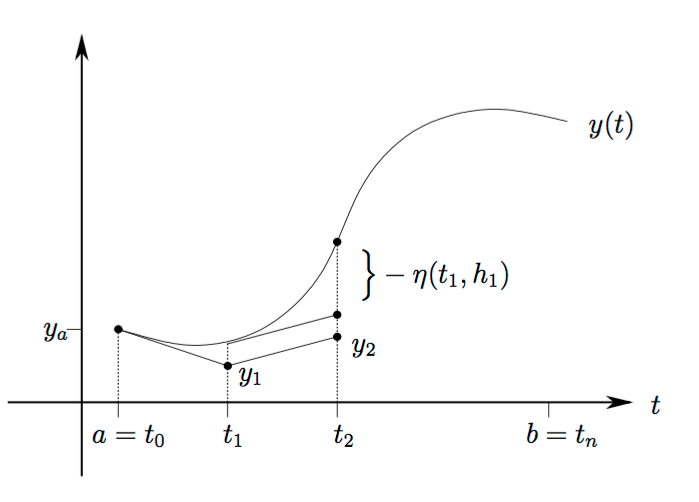
\includegraphics[width=0.50\textwidth]{Pictures/Verfahrensfehler.png} %Bild 1
	\caption[Procedural Error]{Illustration of the Procedural Errors of an One-Step-Scheme.~ \cite{NumerikSkript}}
	\label{fig: Procedural Error}
\end{figure}
\noindent
We now want to use the definitions \ref{def: Procedural Error} to calculate the Order of Consistency of the Euler-Scheme.\\
Starting point is the system \eqref{eqn: Lorentz-Newton}. Thereby we focus on the equation for $u^{\mu}$, since $x^{\mu}$ can be easily integrated from $u^{\mu}$.
Following Definition \ref{def: Procedural Error} we have
\beq
y = u^{\mu}. \nn \\
\eeq
We get
\beq
\label{eqn: eta u}
\eta(\tau, h) = u^{\mu}(\tau_i) + h f^{\mu}(x^{\nu}, u^{\nu}) - u^{\mu}(\tau_{i+1}).
\eeq
The last term can be calculated with a Taylor-expansion analogously to \eqref{eqn: Taylor}.
\beq
\label{eqn: Taylor u}
u^{\mu}(\tau_{i+1}) =  u^{\mu}(\tau_i) + h~\frac{\dm u^{\mu}}{\dm \tau} \Big |_{s=\tau_i}  + h^2~\frac{\dm^2 u^{\mu}}{\dm \tau^2} \Big |_{s=\tau_i}.
\eeq
Plugging in \eqref{eqn: Taylor u} in \eqref{eqn: eta u} yields
\beq
\bal
\eta(\tau, h) &= u^{\mu}(\tau_i) + h\frac{\dm u^{\mu}}{\dm \tau}  - u^{\mu}(\tau_{i+1}) \\
\stackrel{ \eqref{eqn: Taylor u}}{\Longrightarrow}\eta(\tau, h) &= u^{\mu}(\tau_i) + h\frac{\dm u^{\mu}}{\dm \tau}  - u^{\mu}(\tau_i) - h\frac{\dm u^{\mu}}{\dm \tau} - h^2\frac{\dm^2 u^{\mu}}{\dm \tau^2}\\
\Longleftrightarrow\eta(\tau, h) &= \frac{\dm^2 u^{\mu}}{\dm \tau^2}~h^2 ,
\eal
\eeq
since $\frac{\dm u^{\mu}}{\dm \tau} = f^{\mu}(x^{\nu}, u^{\nu})$ holds for the Euler-Scheme. Thus
\beq
|\eta(\tau, h)| \le C h^2 \quad \text{with}~C \coloneqq \frac{1}{2} \max_{\tau \in \mathcal{D}(u^{\mu})}\left| \frac{\dm^2 u^{\mu}}{\dm \tau^2}\right|.
\eeq
$\mathcal{D}(u^{\mu})$ denotes the domain of $u^{\mu}$. Therefore, the Euler-Scheme has an Order of Consistency of one.


%======================== Leap Frog Scheme ========================
\section{Leap-Frog-Scheme}
A definitely better method is the so called \textit{Leap-Frog}-Scheme. One can easily proof that it has an Order of Consistency of two. \\
In contrast to the explicit Euler-Scheme this method has several advantages. For one it is time reversible, i.e. it is possible to reach any previous point in time from every point later in the trajectory. On the other hand the Leap-Frog-Scheme is symplectic, meaning it conserves the phase space volume from which energy and momentum conservation follows. \\
However, one disadvantage is that it's only suited for systems in which the acting force exclusively depends on the current position, but not on the velocity of the particle. This would lead to an implicit equation system which is numerically way more expensive to solve. \\
Thus the differential equation should be of the form
\beq
\frac{\dm^2 x^{\mu}}{\dm \tau^2} = \frac{\dm u^{\mu}}{\dm \tau} = f^{\mu}(x^{\nu}).
\eeq
As we already mentioned, the various methods discretize the differential operators differently
The Leap-Frog-Scheme uses
\beq
\bal
\frac{x^{\mu}_{i+1} - x^{\mu}_i}{h} &= u^{\mu}_{i+\frac{1}{2}}\\
\frac{u^{\mu}_{i+\frac{1}{2}} - u^{\mu}_{i-\frac{1}{2}}}{h} &= f^{\mu}(x^{\nu}_i).
\eal
\eeq
Solving for the new time step yields
\beq
\bal
x^{\mu}_{i+1} &= x^{\mu}_i + h u^{\mu}_{i+\frac{1}{2}}\\
u^{\mu}_{i+\frac{1}{2}} &= u^{\mu}_{i-\frac{1}{2}} + h f^{\mu}(x^{\nu}_i).
\eal
\eeq
\noindent
As we can see, position and velocity are calculated at different times. They are shifted against each other in time by $h = \frac{1}{2}$. \\
But what if we have a system in which the force depends on the velocity ? Are we stuck with expensive implicit methods ? Fortunately not. We can use the \textit{Boris} - Method.
\subsection{Boris-Method}
This method was invented in 1970 by J.P. Boris \cite{boris} and is the standard method for pushing particles in plasma simulations today. We want to solve the Lorentz-Newton equation
\beq
\label{eqn: LorentzNewton}
\bal
\frac{v_{i+\frac{1}{2}} - v_{i - \frac{1}{2}}}{h} &= \frac{q}{m}\left(\vec{E} + \frac{v_{i+\frac{1}{2}} + v_{i - \frac{1}{2}}}{2} \times \vec{B}\right)
\eal
\eeq
Boris noticed, that upon defining
\beq
\label{eqn:vMinusAndPlus}
\bal
\vec{v}_{-} &\coloneqq v_{i - \frac{1}{2}} + \frac{h}{2}\frac{q \vec{E}}{m}\quad\text{and} \\
\vec{v}_{+} &\coloneqq v_{i + \frac{1}{2}} + \frac{h}{2}\frac{q \vec{E}}{m},
\eal
\eeq
one can eliminate the electric field. Plugging in \eqref{eqn:vMinusAndPlus} into \eqref{eqn: LorentzNewton} yields
\beq
\bal
\label{eqn: v+}
\frac{\vec{v}_{+} - \vec{v}_{-}}{h} &= \frac{q}{m} (\vec{v}_{+} + \vec{v}_{-}) \times \vec{B}\\
\Longrightarrow  |\vec{v}_{+} - \vec{v}_{-}| &= \frac{qh}{m} |\vec{v}_{+} + \vec{v}_{-}| B \underbrace{\sin(\vartheta)}_{= 1},
\eal
\eeq
where $\vartheta$ is the angle between $\vec{B}$ and $\vec{v}$. Hence, the steps are
\begin{enumerate}
\item Obtain $\vec{v}_{-}$ by starting from $v_{i - \frac{1}{2}}$ and adding half electric impulse.
\item Use rotation in \eqref{eqn: v+} to obtain $\vec{v}_{+}$ and finally
\item obtain $v_{i + \frac{1}{2}}$ by adding yet another half electric impulse.
\end{enumerate}
\noindent
We now want to do a quick error analysis. We expect the angle of rotation $\theta$ to be close to 
\beq
\omega_ch = \frac{2\pi h}{T} = \frac{qBh}{m},\nn
\eeq
where T is the period.\\
Following the geometrical analysis in ~\cite{Birdsall} illustrated in \ref{fig: borisRotation} and using \eqref{eqn: v+} we find
\beq
\bal
\left|\tan\left(\frac{\theta}{2}\right)\right| &= \frac{\frac{1}{2}|\vec{v}_{+} - \vec{v}_{-}|}{\frac{1}{2}|\vec{v}_{+} + \vec{v}_{-}|} = \frac{qB }{m} \frac{h}{2} = \frac{\omega_c h}{2}\\
\Longrightarrow \theta &= 2\arctan\left(\frac{\omega_c h}{2}\right) = \omega_c h \left(1 - \frac{\omega^2_c h^2}{12} + \ldots \right).
\eal
\eeq
For $\omega_ch < 0.35$ we get an error smaller than $1\%$.
\begin{figure}[H]
	\centering
		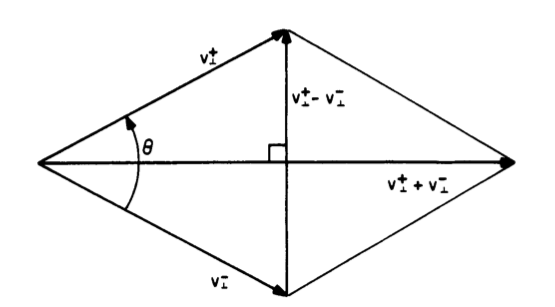
\includegraphics[width=0.50\textwidth]{Pictures/borisRotation.png} 
	\caption[Determination of $\left|\tan\left(\frac{\theta}{2}\right)\right|$ from boris roation]{Determination of $\left|\tan\left(\frac{\theta}{2}\right)\right|$ from boris rotation~\cite{Birdsall}}
	\label{fig: borisRotation}
\end{figure}
\noindent
Up to now one question remains unanswered. How do we calculate the rotation effectively? To answer this, we use figure \ref{fig: borisProjection}.
\begin{figure}[H]
	\centering
		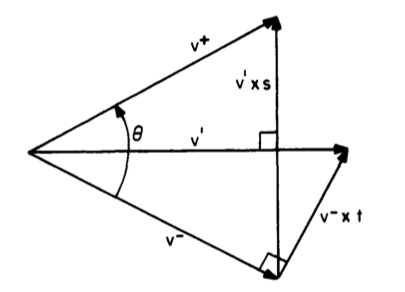
\includegraphics[width=0.50\textwidth]{Pictures/borisProjection.png} 
	\caption[Velocity space showing the rotation from $\vec{v}_{-}$ to $\vec{v}~'$]{Velocity space showing the rotation from $\vec{v}_{-}$ to $\vec{v}~'$. The velocities shown are projections of the total velocities onto the plane perpendicular to $\vec{B}$. ~\cite{Birdsall}}
	\label{fig: borisProjection}
\end{figure}
\noindent
What we want is a vector, which is parallel to $\vec{v}_{+} - \vec{v}_{-}$. Its magnitude is yet to be determined. However, if we can find a vector $\vec{v}~'$ which is perpendicular to $\vec{v}_{+} - \vec{v}_{-}$, then $\vec{v}~' \times \vec{s}$, where $\vec{s} \propto \vec{B}$, is exactly what we need.\\
Upon defining
\beq
\vec{t} \coloneqq -\frac{\vec{B}}{B} \tan\left(\frac{\theta}{2}\right) = \frac{q\vec{B}h}{2m},
\eeq
we obtain $\vec{v}~'$ from
\beq
\vec{v}~' = \vec{v}_{-} + \vec{v}_{-} \times \vec{t}.
\eeq
Now $\vec{v}~' $ is perpendicular to  $\vec{v}_{+} - \vec{v}_{-}$. Finally we need a vector $\vec{s} \propto \vec{B}$ wich magnitude is determined by the constraint $|\vec{v}_{+}|= |\vec{v}_{-}|$. Using half angle formulas we find 
\beq
\vec{s} = \frac{2\vec{t}}{1+t^2}.
\eeq
Hence
\beq
\vec{v}_{+}= \vec{v}_{-} + \vec{v}~' \times \vec{s}.
\eeq

%======================== Nystr�m Scheme ========================
\section{Nystr�m-Scheme}

%======================== Adaptive Timestep control ========================
\section{Adaptive Timestep Control}


%======================== Interpolations ========================
%===========================================================
\chapter{Interpolations}

%======================== Linear interpolation of Trajectories ========================
\section{Linear interpolation of Trajectories}
\label{sec: Interpolation of Trajectories}
The previously presented methods calculate the particle trajectory solely at discrete points in time $x_i^{\mu}(\tau)$. Calculating Li�nard-Wiechert fields according to equation \eqref{eqn: Li�nard-Wiechert} however, requires the intersection point of the trajectory with the backward lightcone of the observation point. 
In most cases the calculated points of the trajectory are not lying directly on the lightcone, so we need a procedure to calculate the intersection point exactly.\\
The simplest solution is a linear interpolation between the last point inside and the first point outside the lightcone. Figure \ref{fig: Interpolation} illustrates the situation.
\begin{figure}[H]
	\centering
		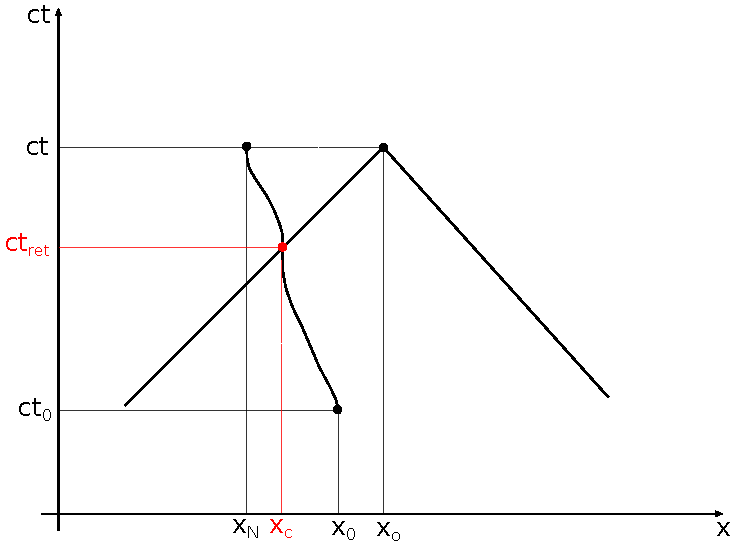
\includegraphics[width=0.80\textwidth]{Pictures/LightconeNew.pdf}
	\caption[Interpolation of Trajectories]{Minkowski space showing the particle trajectory with starting point $x^{\mu}_0(t_0)$ and last point $x^{\mu}_N(t)$. The observation point $x^{\mu}_o(t)$ with its backward lightcone is also shown. If we want to calculate the Li�nard-Wiechert fields at the observation point $x^{\mu}_o(t)$, we need the intersection point $x^{\mu}_c(t_{ret})$ of the trajectory with the backward lightcone. }
	\label{fig: Interpolation}
\end{figure}
\noindent
Thereto let $x_j^{\mu} \in \mathbb{R}^{3+1}$ be the last point inside and $x_{j+1}^{\mu} \in \mathbb{R}^{3+1}$ the first point outside the lightcone. Further let $x_{c}^{\mu} \in \mathbb{R}^{3+1}$ be the intersection point of interest then we get
\beq
\label{eqn: linInt}
x_c^{\mu} = x_j^{\mu} + \lambda ~\left(x_{j+1}^{\mu} - x_j^{\mu}\right),
\eeq
where $\lambda \in [0,1]$. Due to the finite speed of light the intersection point $x_c^{\mu}$ needs to fulfill
\beq
\label{eqn: constraint}
\left| \vec{x}_o(t) - \vec{x}_c(t_{ret})\right| = c~(t - t_{ret}) \Longleftrightarrow (x_o - x_c)_{\mu} (x_o - x_c)^{\mu} = 0.
\eeq
Thereby $x_o^{\mu} \in \mathbb{R}^{3+1}$ denotes the observation point where the fields shall be calculated. Note, that on the left hand side of \eqref{eqn: constraint} only spatial components of the respective four vectors are used. \\
Plugging in \eqref{eqn: linInt} in \eqref{eqn: constraint} yields

\begin{multline}
\label{eqn: quadEq}
\lambda^2 (x_{j+1} - x_j)_{\mu}(x_{j+1} - x_j)^{\mu} + \lambda~2(x_{j+1} - x_j)_{\mu}(x_j - x_o)^{\mu} + (x_j)_{\mu}(x_j)^{\mu} \\ + (x_o)_{\mu}(x_o)^{\mu} - 2(x_j)_{\mu}(x_o)^{\mu}  = 0.
\end{multline}
We define
\beq
\bal
a &\coloneqq (x_{j+1} - x_j)_{\mu}(x_{j+1} - x_j)^{\mu}\\
b &\coloneqq 2(x_{j+1} - x_j)_{\mu}(x_j - x_o)^{\mu} \\
c &\coloneqq (x_j)_{\mu}(x_j)^{\mu} + (x_o)_{\mu}(x_o)^{\mu} - 2(x_j)_{\mu}(x_o)^{\mu}. \nn
\eal
\eeq
In general the quadratic equation \eqref{eqn: quadEq} in $\lambda$ has two solutions
\beq
\lambda_{1/2} = \frac{-b \pm \sqrt{b^2 - 4ac}}{2a}. \nn
\eeq
One denotes the intersection point with the backward lightcone, the other one with the forward lightcone. Since  $\lambda \in [0,1]$ we are only interested in the larger one. 
\beq
\lambda_{1/2} = \frac{-b + \sqrt{b^2 - 4ac}}{2a}. \nn
\eeq
Plugging in $\lambda$ in \eqref{eqn: linInt} gives the desired intersection point.

%======================== trilinear interpolation of fields ========================
\section{Trilinear Interpolation of Fields}


%======================== Hybrid Fields ========================
%===========================================================
\chapter{FDTD}
In this section we introduce the concept of hybrid fields and how this approach reduces the numerical complexity from $N^2$ to $N$.\\
Usually the numerical complexity of multi particle simulation is $N^2$, due to the interaction between each particle. In our case we need $N$ push operations for the particles. One push for each particle. In order to do that, however, we need to solve equation \eqref{eqn: Lorentz-Newton} and therefore all Li�nard-Wiechert fields from the other $N-1$ particles are needed. This results in $N(N-1)$ calculations for each time step, period. If we want to calculate the Li�nard-Wiechert fields, we also need to store all positions from all particles, as explained in section \ref{sec: Interpolation of Trajectories}. For a few particles such simulations are effortlessly feasible. But with increasing particle numbers such simulations may not just require more and more memory capacity but also become so time consuming that at some point we simply can not do them anylonger. That's where the hybrid field model comes in. Instead of calculating the Li�nard-Wiechert fields at every time step for all particles at all grid points we save them onto the grid and propagate them through the grid using Maxwell equations. How that works in detail is explained in the following sections. 

%%======================== Maxwell Equations ========================
%\section{Maxwell-Equations}
% MISSING: Which one to use ? For Maxwell Pusher  the vacuum equations are suffice. For UPML we need the ones in anisotropic media
%The Maxwell equations are the foundation of the classical electromagnetism and describe how the electric field $\vec{E} \in \mathbb{R}^3$ and the magnetic field $\vec{H} \in \mathbb{R}^3$ are generated by charges and currents respectively and how they evolve over time in space in presence of one another. In homogenous and isotropic media the Maxwell Equations read
%\beq
%\label{eqn: maxwellEq}
%\bal
%\epsilon_0\epsilon_r \vec{\nabla} \vec{E} &= \rho \\
%\mu_0\mu_r \vec{\nabla} \vec{B} &= 0\\
%\vec{\nabla} \times \vec{E} &= - \mu_0\mu_r \frac{\del \vec{B}}{\del t}\\
%\vec{\nabla} \times \vec{H} &=  \epsilon_0\epsilon_r \frac{\del \vec{E}}{\del t} + \sigma \vec{E},
%\eal
%\eeq
%where $\epsilon_0 $ and $\epsilon_r$ are the vacuum and the relative electric permeability respectively. Same holds for $\mu_0$ and $\mu_r $ for magnetic materials.
%$\rho$ denotes the current density of the electric source and $\sigma$ the electric conductivity. \\
%To solve the Maxwell equations numerically we need to discretize them first. The most robust and reliable way of doing this is with the \textit{Yee-Algorithm}. 

%======================== Yee Scheme ========================
\section{The Yee-Scheme}
\label{sec: Yee-Scheme}
In this section we talk about how to solve the Maxwell Equations \eqref{eqn: maxwellEq} and how to propagate the fields on a numerical grid. We thereby focus on the Maxwell Equations in vacuum, i.e. $\rho = \vec{j} = 0$. As can be seen in the Li�nard-Wiechert formula \eqref{eqn: Li�nard-Wiechert} there is a singularity for the field values at the particle position itself. Thus, we just want to propagate fields far away from the source, which is explained in more detail later.\\
\newline 
To push the fields on the grid. i.e solving for the fields at the next time step, we use the Yee - Scheme introduced by \textit{Kane Yee} in 1966 \cite{Yee66} to discretize the Maxwell Equations. Each point on the discretized grid is represented as a tuple $(i,j,k)$. One index for each dimension $(x,y,z)$. The distance between the grid points are $(\Delta x, \Delta y, \Delta z)$ respectively. $h$ denotes the time discretization as before. In order to have finite central differences rather than plain finite differences, the evaluation of $\vec{E}$ and $\vec{H}$ components are shifted in time about $\frac{h}{2}$ against each other. To have the same benefits for the rotation, the $\vec{E}$ and $\vec{H}$ components are shifted in space as well, as it's illustrated in figure \ref{fig: YeeBox}.
\begin{figure}[H]
	\centering
		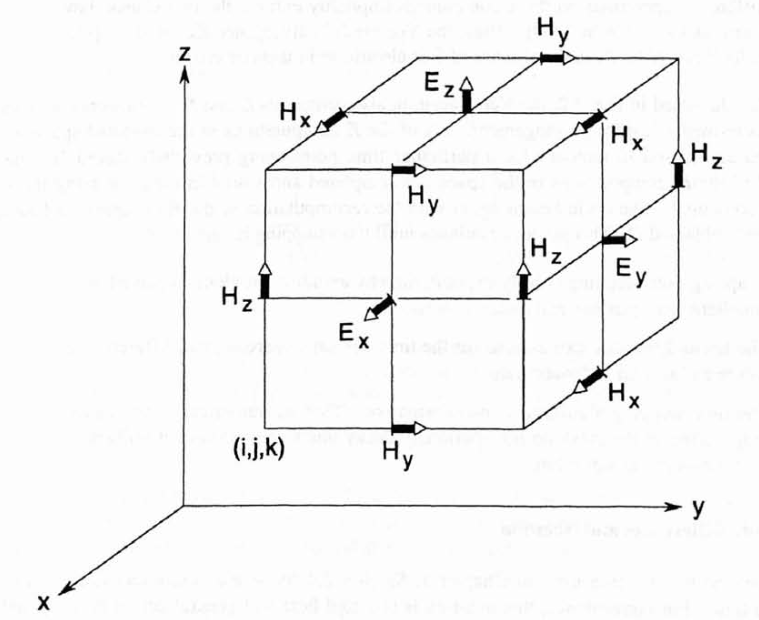
\includegraphics[width=0.70\textwidth]{Pictures/YeeBox.png} 
	\caption[Yee-Box]{An illustration of a so called Yee-Box which is used to solve the curl Maxwell Equations. Shown are the positions of the electric and magnetic field vector components about a cubic unit cell of the Yee space lattice.The Yee algorithm centers its E and H components in three- dimensional space so that every E component is surrounded by four circulating H components, and every H component is surrounded by four circulating E components.\cite{Taflove}.}
	\label{fig: YeeBox}
\end{figure}
The discrete Maxwell equations then read
%\vec{E}^{n+\frac{1}{2}}_{(i,j,k)}
\beq
\label{eqn: discreteMaxwellEq}
\bal
\frac{\vec{E}\Bigr|^{n+\frac{1}{2}}_{(i,j,k)} - \vec{E}\Bigr|^{n-\frac{1}{2}}_{(i,j,k)}}{h} = \vec{\nabla}^{-} \times \vec{H}\Bigr|^{n}_{(i,j,k)},\\
\frac{\vec{H}\Bigr|^{n+1}_{(i,j,k)} - \vec{H}\Bigr|^{n}_{(i,j,k)}}{h} = \vec{\nabla}^{+} \times \vec{E}\Bigr|^{n+\frac{1}{2}}_{(i,j,k)}.
\eal
\eeq
The operators $\vec{\nabla}^{-}$ and $\vec{\nabla}^{+}$ act on a discretized vector field $F\Bigr|_{(i,j,k)}:\mathbb{R}^3 \to \mathbb{R}$ as follows
\beq
%F_{(i + 1,j,k)} - F_{(i,j,k)}{\Delta x}
\vec{\nabla}^{-} F\Bigr|_{(i,j,k)} \coloneqq \left( \frac{F\Bigr|_{(i,j,k)} - F\Bigr|_{(i-1,j,k)}}{\Delta x}, \frac{F\Bigr|_{(i,j,k)} - F\Bigr|_{(i,j-1,k)}}{\Delta y}, \frac{F\Bigr|_{(i,j,k1)} - F\Bigr|_{(i,j,k-1)}}{\Delta z}\right)^{T},\\
\vec{\nabla}^{+} F\Bigr|_{(i,j,k)} \coloneqq \left( \frac{F\Bigr|_{(i + 1,j,k)} - F\Bigr|_{(i,j,k)}}{\Delta x}, \frac{F\Bigr|_{(i,j + 1,k)} - F\Bigr|_{(i,j,k)}}{\Delta y}, \frac{F\Bigr|_{(i,j,k+1)} - F\Bigr|_{(i,j,k)}}{\Delta z}\right)^{T},
\eeq
where $T$ denotes the transpose as usual. The spatial positions where $\vec{E}$ and $\vec{H}$ components will be calculated are given by
\beq
\bal
\vec{E}\Bigr|_{(i,j,k)} &= 
\begin{pmatrix}
E_{x}\left[\left(i+\frac{1}{2}\right)\Delta x, j\Delta y,  k\Delta z\right]\\[0.5em]
E_{y}\left[i \Delta x, \left(j+\frac{1}{2}\right)\Delta y,  k\Delta z\right]\\[0.5em]
E_{z}\left[i\Delta x, j\Delta y,  \left(k+\frac{1}{2}\right)\Delta z\right]
\end{pmatrix}, \\
\vec{H}\Bigr|_{(i,j,k)} &= 
\begin{pmatrix}
H_{x}\left[i\Delta x, \left(j+\frac{1}{2}\right)\Delta y, \left(k+\frac{1}{2}\right)\Delta z\right]\\[0.5em]
H_{y}\left[\left(i+\frac{1}{2}\right) \Delta x, j\Delta y,  \left(k+\frac{1}{2}\right)\Delta z\right]\\[0.5em]
H_{z}\left[\left(i+\frac{1}{2}\right)\Delta x, \left(j+\frac{1}{2}\right)\Delta y, \Delta z\right]
\end{pmatrix}.
\eal
\eeq
%======================== Dispersion Relation ========================
\section{Numeric Dispersion Relation}
\label{sec: DispersionRelation}
By discretizing the numerical grid, the dispersion relation of light also changes. To study this effect we need to solve the discretized Maxwell Equations \eqref{eqn: discreteMaxwellEq}. Without loss of generality we choose the Ansatz of a TMz-mode, i.e. $H_z = 0$ and $E_z \neq 0$:
\beq
\bal
\label{eqn: TMz-mode}
E_z\Bigr|_{(i,j,k)}^{n} &= E_{z_0} \exp\left\{\hat{i}\left(\tilde{k}_x i\Delta x + \tilde{k}_y i\Delta y - \omega nh\right)\right\}\\
H_x\Bigr|_{(i,j,k)}^{n} &= H_{x_0} \exp\left\{\hat{i}\left(\tilde{k}_x i\Delta x + \tilde{k}_y i\Delta y - \omega nh\right)\right\}\\
H_y\Bigr|_{(i,j,k)}^{n} &= H_{y_0} \exp\left\{\hat{i}\left(\tilde{k}_x i\Delta x + \tilde{k}_y i\Delta y - \omega nh\right)\right\},
\eal
\eeq
where $\hat{i}$ denotes the imaginary unit and $\tilde{k}_x$, $\tilde{k}_y$ the x- and y-components of the wave vector. Using TMz-mode, \eqref{eqn: discreteMaxwellEq} also simplifies to
\beq
\bal
\label{eqn: simplifiedMaxwellEq}
\frac{E_z\Bigr|^{n+\frac{1}{2}}_{(i,j,k)} - E_z\Bigr|^{n-\frac{1}{2}}_{(i,j,k)}}{h} &= \left( \frac{H_y\Bigr|^{n}_{(i,j,k)} - H_y\Bigr|^{n}_{(i-1,j,k)}}{\Delta x} - \frac{H_x\Bigr|^{n}_{(i,j,k)} - H_x\Bigr|^{n}_{(i,j-1,k)}}{\Delta y}\right)\\
\frac{H_x\Bigr|^{n+1}_{(i,j,k)} - H_x\Bigr|^{n}_{(i,j,k)}}{h} &= - \left(\frac{E_z\Bigr|^{n+\frac{1}{2}}_{(i,j+1,k)} - E_z\Bigr|^{n+\frac{1}{2}}_{(i,j,k)}}{\Delta y}\right)\\
\frac{H_y\Bigr|^{n+1}_{(i,j,k)} - H_y\Bigr|^{n}_{(i,j,k)}}{h} &= \left(\frac{E_z\Bigr|^{n+\frac{1}{2}}_{(i+1,j,k)} - E_z\Bigr|^{n+\frac{1}{2}}_{(i,j,k)}}{\Delta x}\right).
\eal
\eeq
Upon substituting \eqref{eqn: TMz-mode} in \eqref{eqn: simplifiedMaxwellEq} and after some manipulation we find
\beq
E_{z_0}\sin\left(\frac{\omega h}{2}\right) &=& h\left[\frac{H_{x_0}}{\Delta y}\sin\left(\frac{\tilde{k}_y \Delta y}{2}\right) - \frac{H_{y_0}}{\Delta x}\sin\left(\frac{\tilde{k}_x \Delta x}{2}\right)\right]\\[0.5em]
\label{eqn: Hx0}
H_{x_0} &=& \frac{h E_{z_0}}{\Delta y} \frac{\sin\left(\frac{\tilde{k}_y \Delta y}{2}\right)}{\sin\left(\frac{\omega h}{2}\right)}\\[0.5em]
\label{eqn: Hy0}
H_{y_0} &=& \frac{h E_{z_0}}{\Delta x} \frac{\sin\left(\frac{\tilde{k}_x \Delta x}{2}\right)}{\sin\left(\frac{\omega h}{2}\right)}.
\eeq
Plugging in \eqref{eqn: Hx0} and \eqref{eqn: Hy0} in \eqref{eqn: simplifiedMaxwellEq} we obtain the numerical dispersion relation
\beq
\bal
\label{eqn: dispersionRelation2D}
\left[\frac{1}{h}\sin\left(\frac{\omega h}{2}\right)\right]^2 = \left[\frac{1}{\Delta x}\sin\left(\frac{\tilde{k}_x \Delta x}{2}\right)\right]^2  + \left[\frac{1}{\Delta y}\sin\left(\frac{\tilde{k}_y \Delta y}{2}\right)\right]^2 \\
\eal
\eeq
For the one dimensional case \eqref{eqn: dispersionRelation2D} reduces to 
\beq
\label{eqn: dispersionRelation1D}
\omega h = 2\arcsin\left(\frac{\Delta t}{\Delta x} \sin\left(\frac{\tilde{k}_x \Delta x}{2}\right)\right),
\eeq
which is still more complicated than the analytic dispersion relation
\beq
\omega = k.
\eeq
In figure \ref{fig: dispersionRelation} both the analytical and the numerical dispersion relation are plotted. Equation \eqref{eqn: dispersionRelation1D} has a maximum at 
\beq
\bal
\tilde{k}_x^{max} &= \frac{\pi}{\Delta x}\\
\Longleftrightarrow\lambda_x^{max} &= 2 \Delta x.
\eal
\eeq
$\tilde{k}_x^{max}$ is the largest possible wavevector - also called \textit{Nyquist Limit} for a numerical grid with resolution $\Delta x$, or $\Delta y$, $\Delta z$ respectively. At this wavevector, the group velocity 
\beq
v_g = \frac{\del \tilde{k}_x}{\del \omega}\Bigr|_{\tilde{k} = \tilde{k}^{max}} = 0.
\eeq
vanishes, instead of propagating with speed of light. That means, that the Yee-Scheme is only valid for wavelength $\lambda \ll \lambda^{max}$.
\begin{figure}[H]
	\centering
		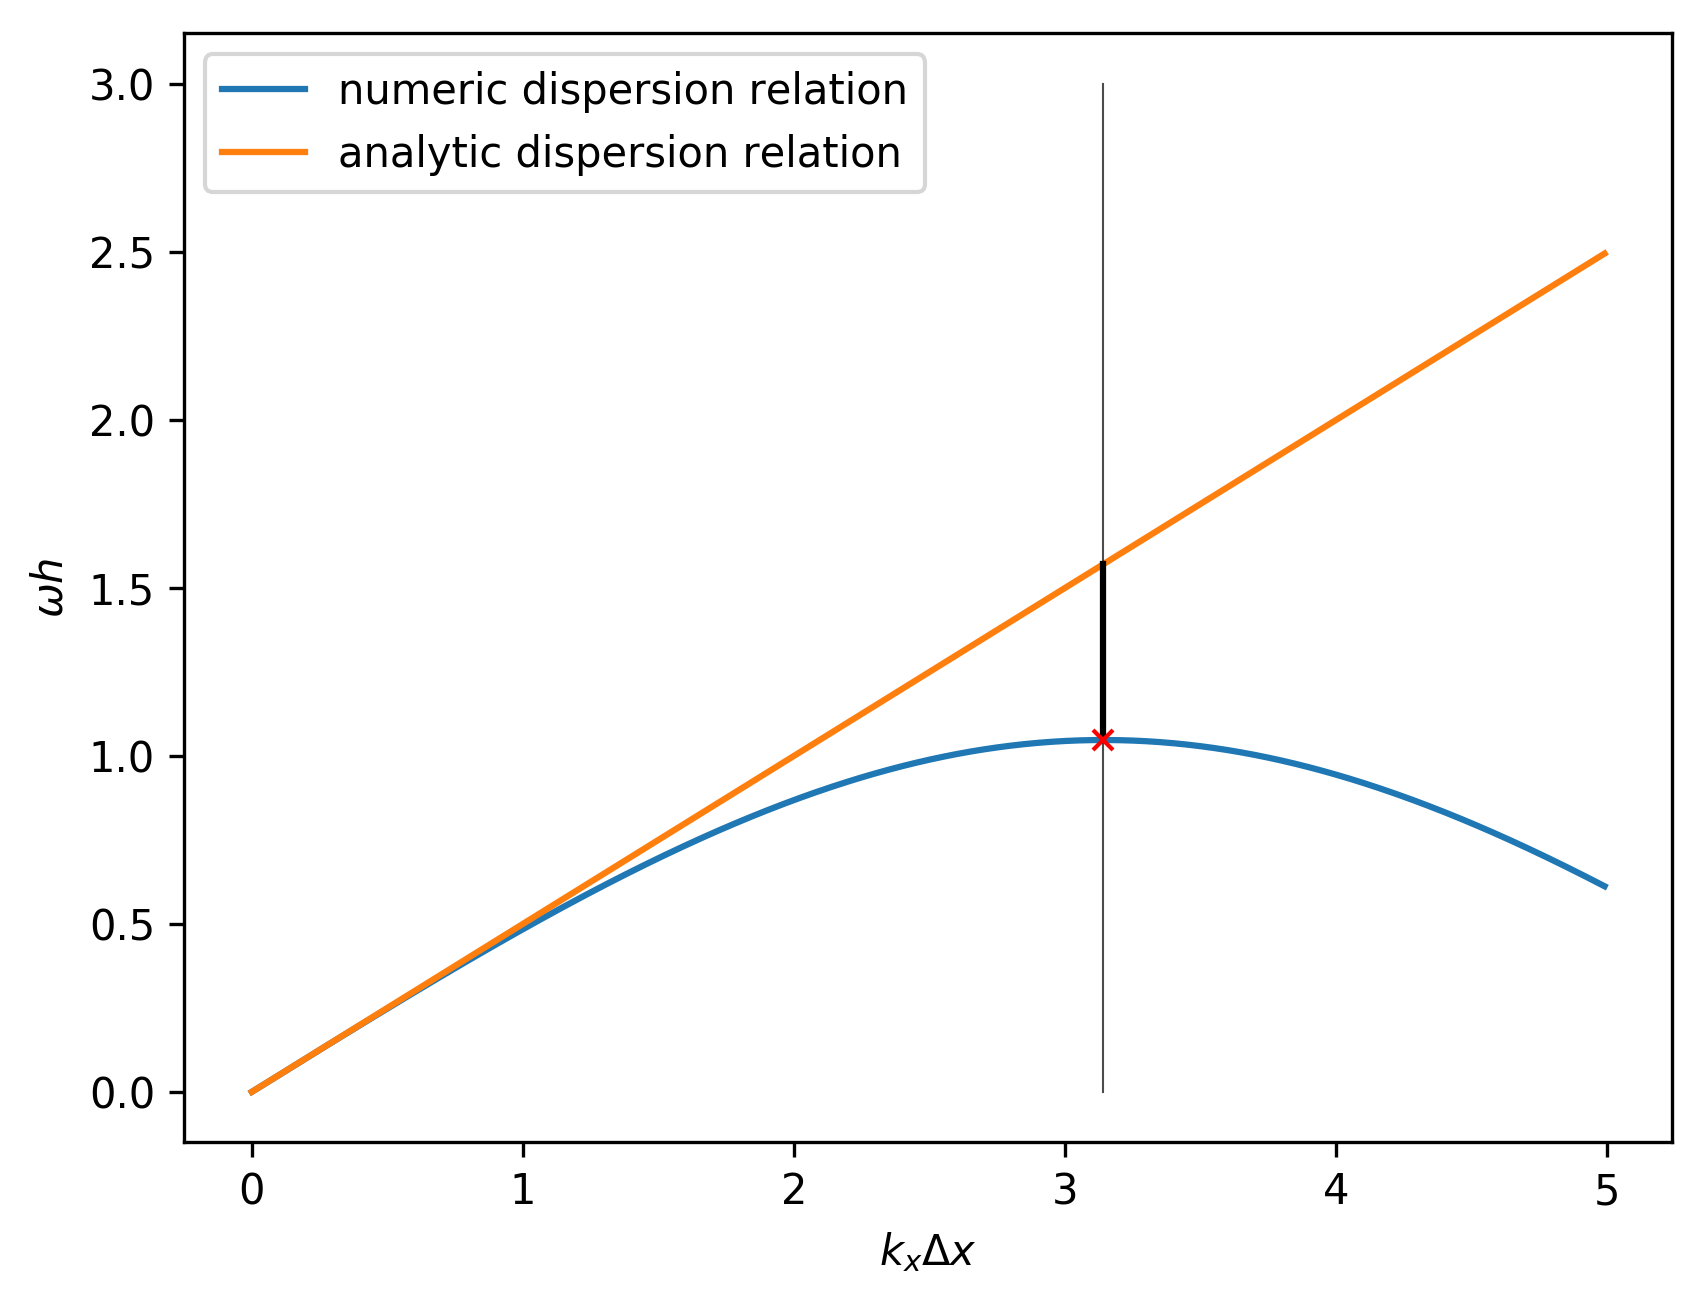
\includegraphics[width=0.70\textwidth]{Pictures/dispersionRelation.png} 
	\caption[Comparison of numerical and analytical dispersion relation of discretized Maxwell Equations with Yee Scheme]{Comparison of numerical and analytical dispersion relation of discretized Maxwell Equations with Yee Scheme. We used $c \equiv 1$ and $\frac{\Delta t}{\Delta x} \equiv \frac{1}{2}$.}
	\label{fig: dispersionRelation}
\end{figure}


%============== Hybrid Field Approach ===================
%================================================

\chapter{Hybrid Field Approach}
After having discussed the fundamentals, we now want to dive into practice. In section \ref{sec: Yee-Scheme} we learned how to store and propagate the fields on a numerical grid. In section \ref{sec: lw-potentials} we derived an analytical expression, of how to calculate the fields of a moving charged particle. We also observed that there is a singularity in \eqref{eqn: Li�nard-Wiechert} at the particle position itself. That means, that the fields will vary strongly in  a vicinity of the particle and can not be resolved correctly on the grid, as discussed in section \ref{sec: DispersionRelation}. Hence, it seems plausible to separate the simulation area into appropriate Near - and Farfield areas. Within the Nearfield area of a particle, its fields will \textbf{not} be stored on the grid. We then do not need to worry about the singularity. Only Farfields from other particles, propagated into the Nearfield area will be further propagated and stored on the grid. Possible interactions with other particles within the Nearfield area will be caluclated analytically from \eqref{eqn: Li�nard-Wiechert}. \\
Farfields will be stored on the grid and propagated with the Yee-Scheme \eqref{eqn: discreteMaxwellEq}.
%======================== Near and Far- Fields ========================
\section{Near-and Farfields}
Before we can separate the simulation area into Near - and Farfields, we need to initialize a grid. We divide the grid in \texttt{numberBoxesInX}, \texttt{numberBoxesInY} and \texttt{numberBoxesInZ} boxes, each of which has \texttt{numberOfGridPointsForBoxInX}, \texttt{numberOfGridPointsForBoxInY} and \texttt{numberOfGridPointsForBoxInZ} length, which leaves us with a total 
\begin{lstlisting}
numberOfGridPointsInX = numberOfGridPointsForBoxInX * numberOfBoxesInX;
numberOfGridPointsInY = numberOfGridPointsForBoxInY * numberOfBoxesInY;
numberOfGridPointsInZ = numberOfGridPointsForBoxInZ * numberOfBoxesInZ;
\end{lstlisting}
Upon defining the resolution \texttt{dx}, \texttt{dy}, \texttt{dz} the size of the simulation area is then given by 
\begin{lstlisting}
lengthOfSimulationBoxInX = numberOfGridPointsInX * dx;
lengthOfSimulationBoxInY = numberOfGridPointsInY * dy;
lengthOfSimulationBoxInZ = numberOfGridPointsInZ * dz;
\end{lstlisting}
The Nearfield is then defined as the $3 \cdot 3 \cdot 3 = 27$ boxes with the box, containing the particle, in the center. In figure \ref{fig: nearFields} the Nearfields of one and two particles are shown. The Nearfields can of course overlap. The Nearfield box at $(18,18)$ belongs to both particles.
\begin{figure}
\subfigure[]{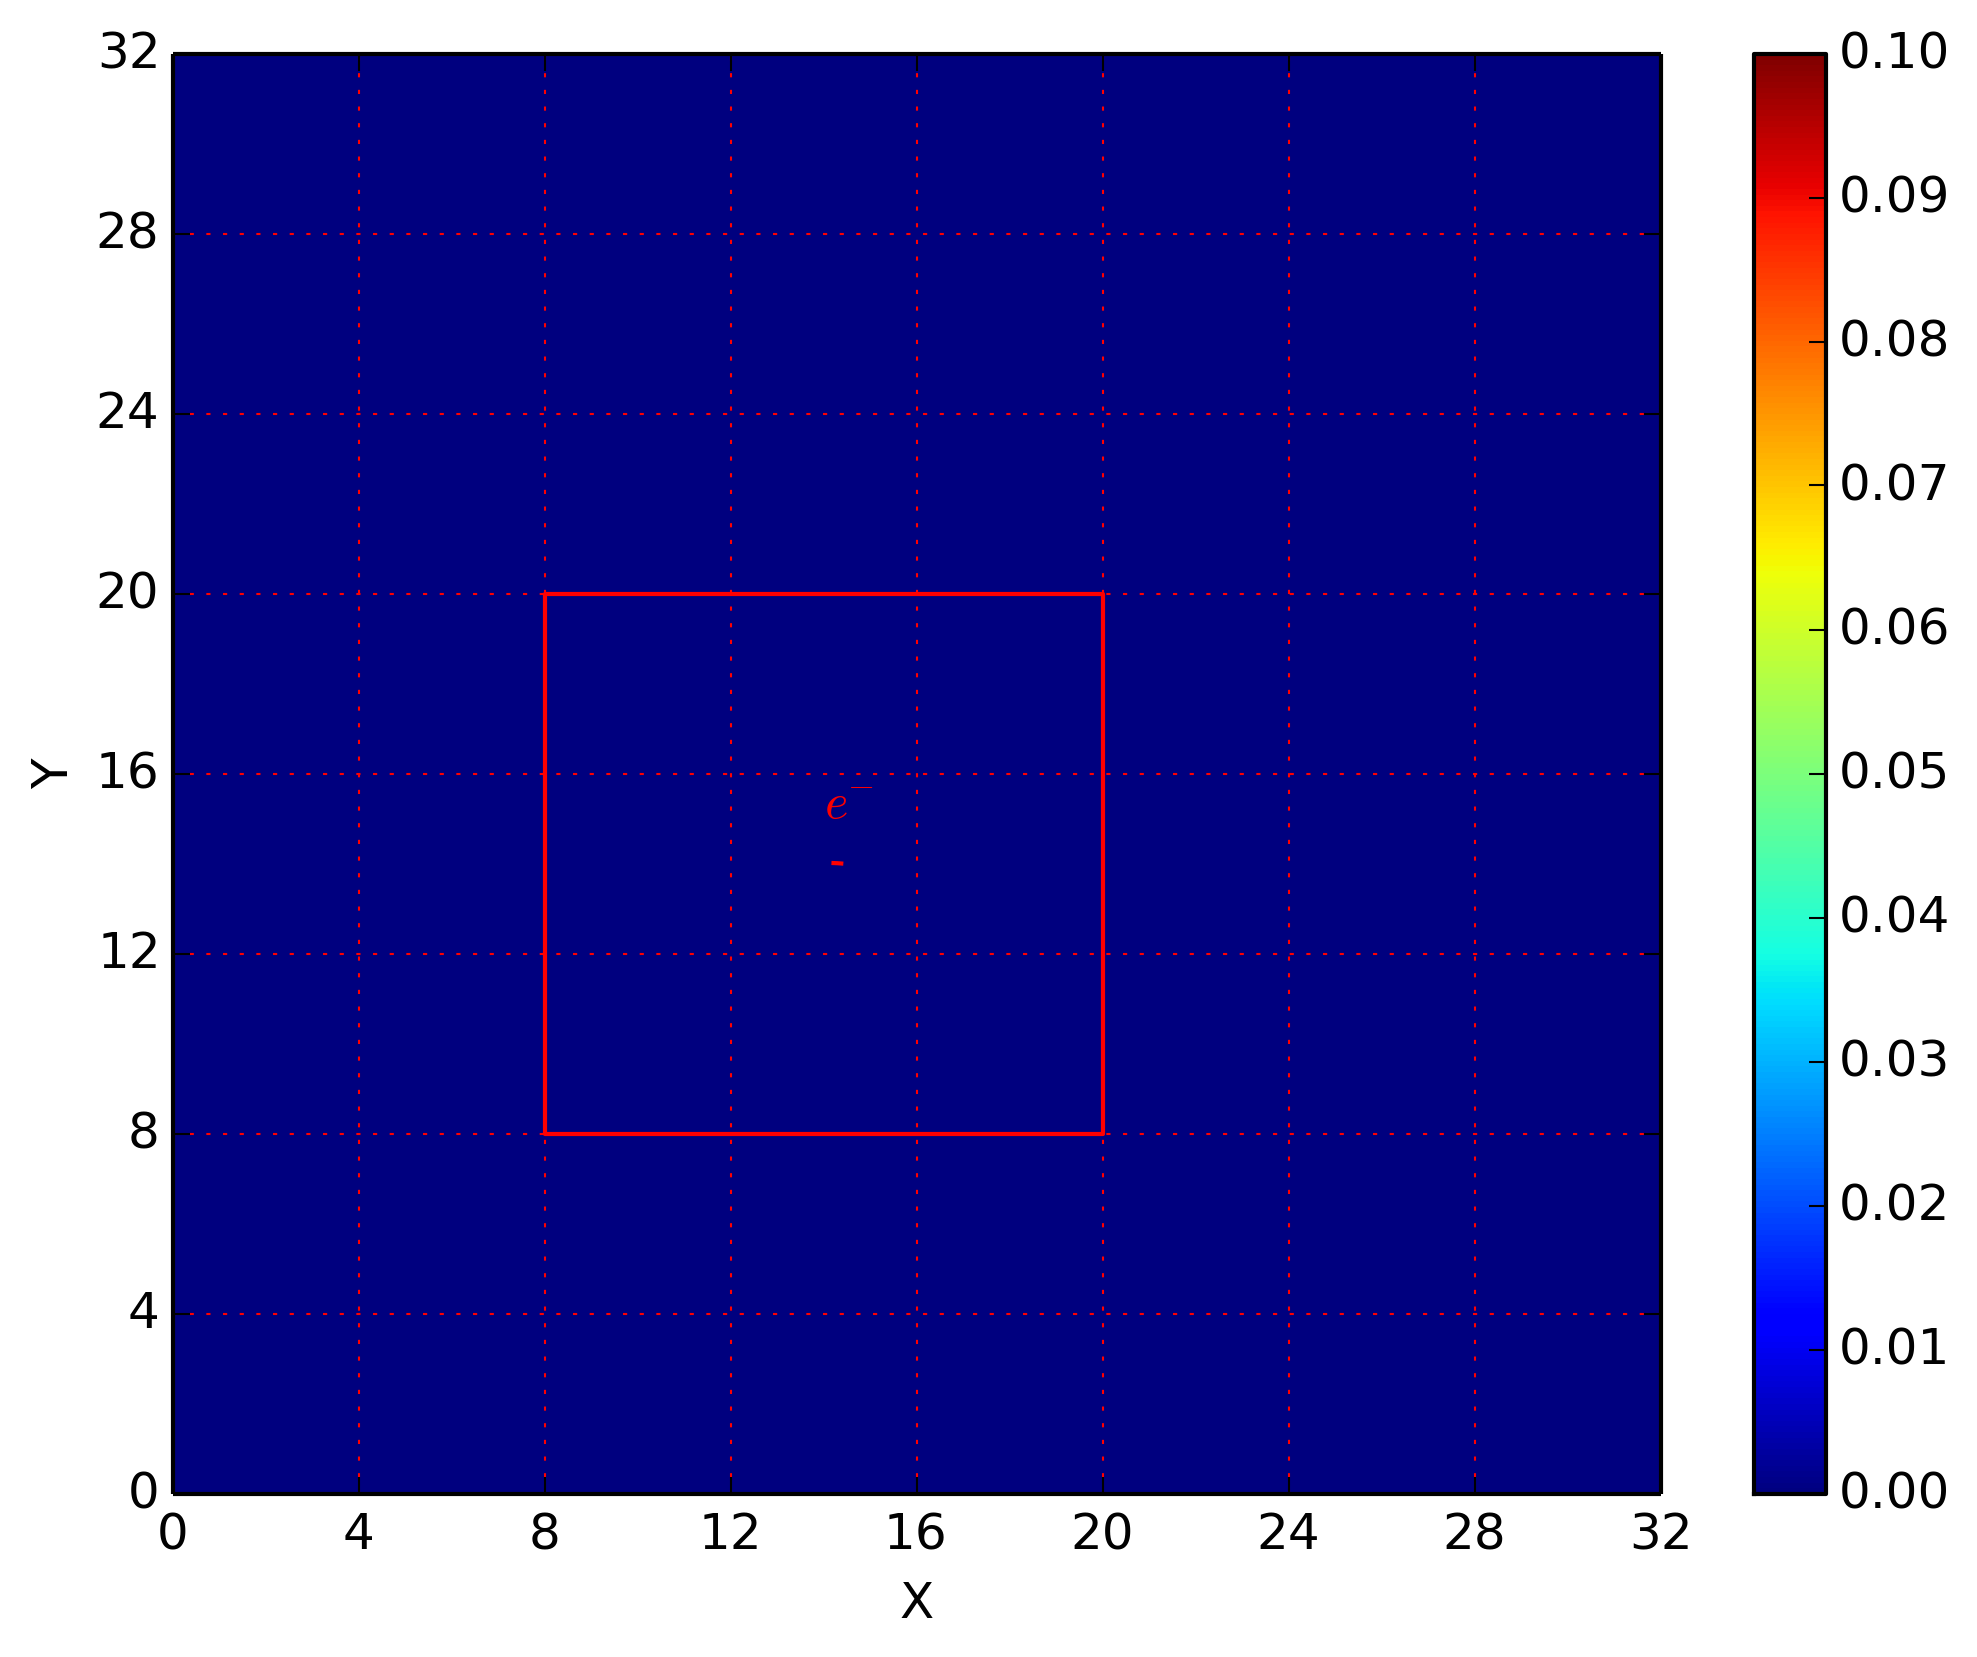
\includegraphics[width=0.49\textwidth]{Pictures/nearFieldOneParticle.png}}\hfill
\subfigure[]{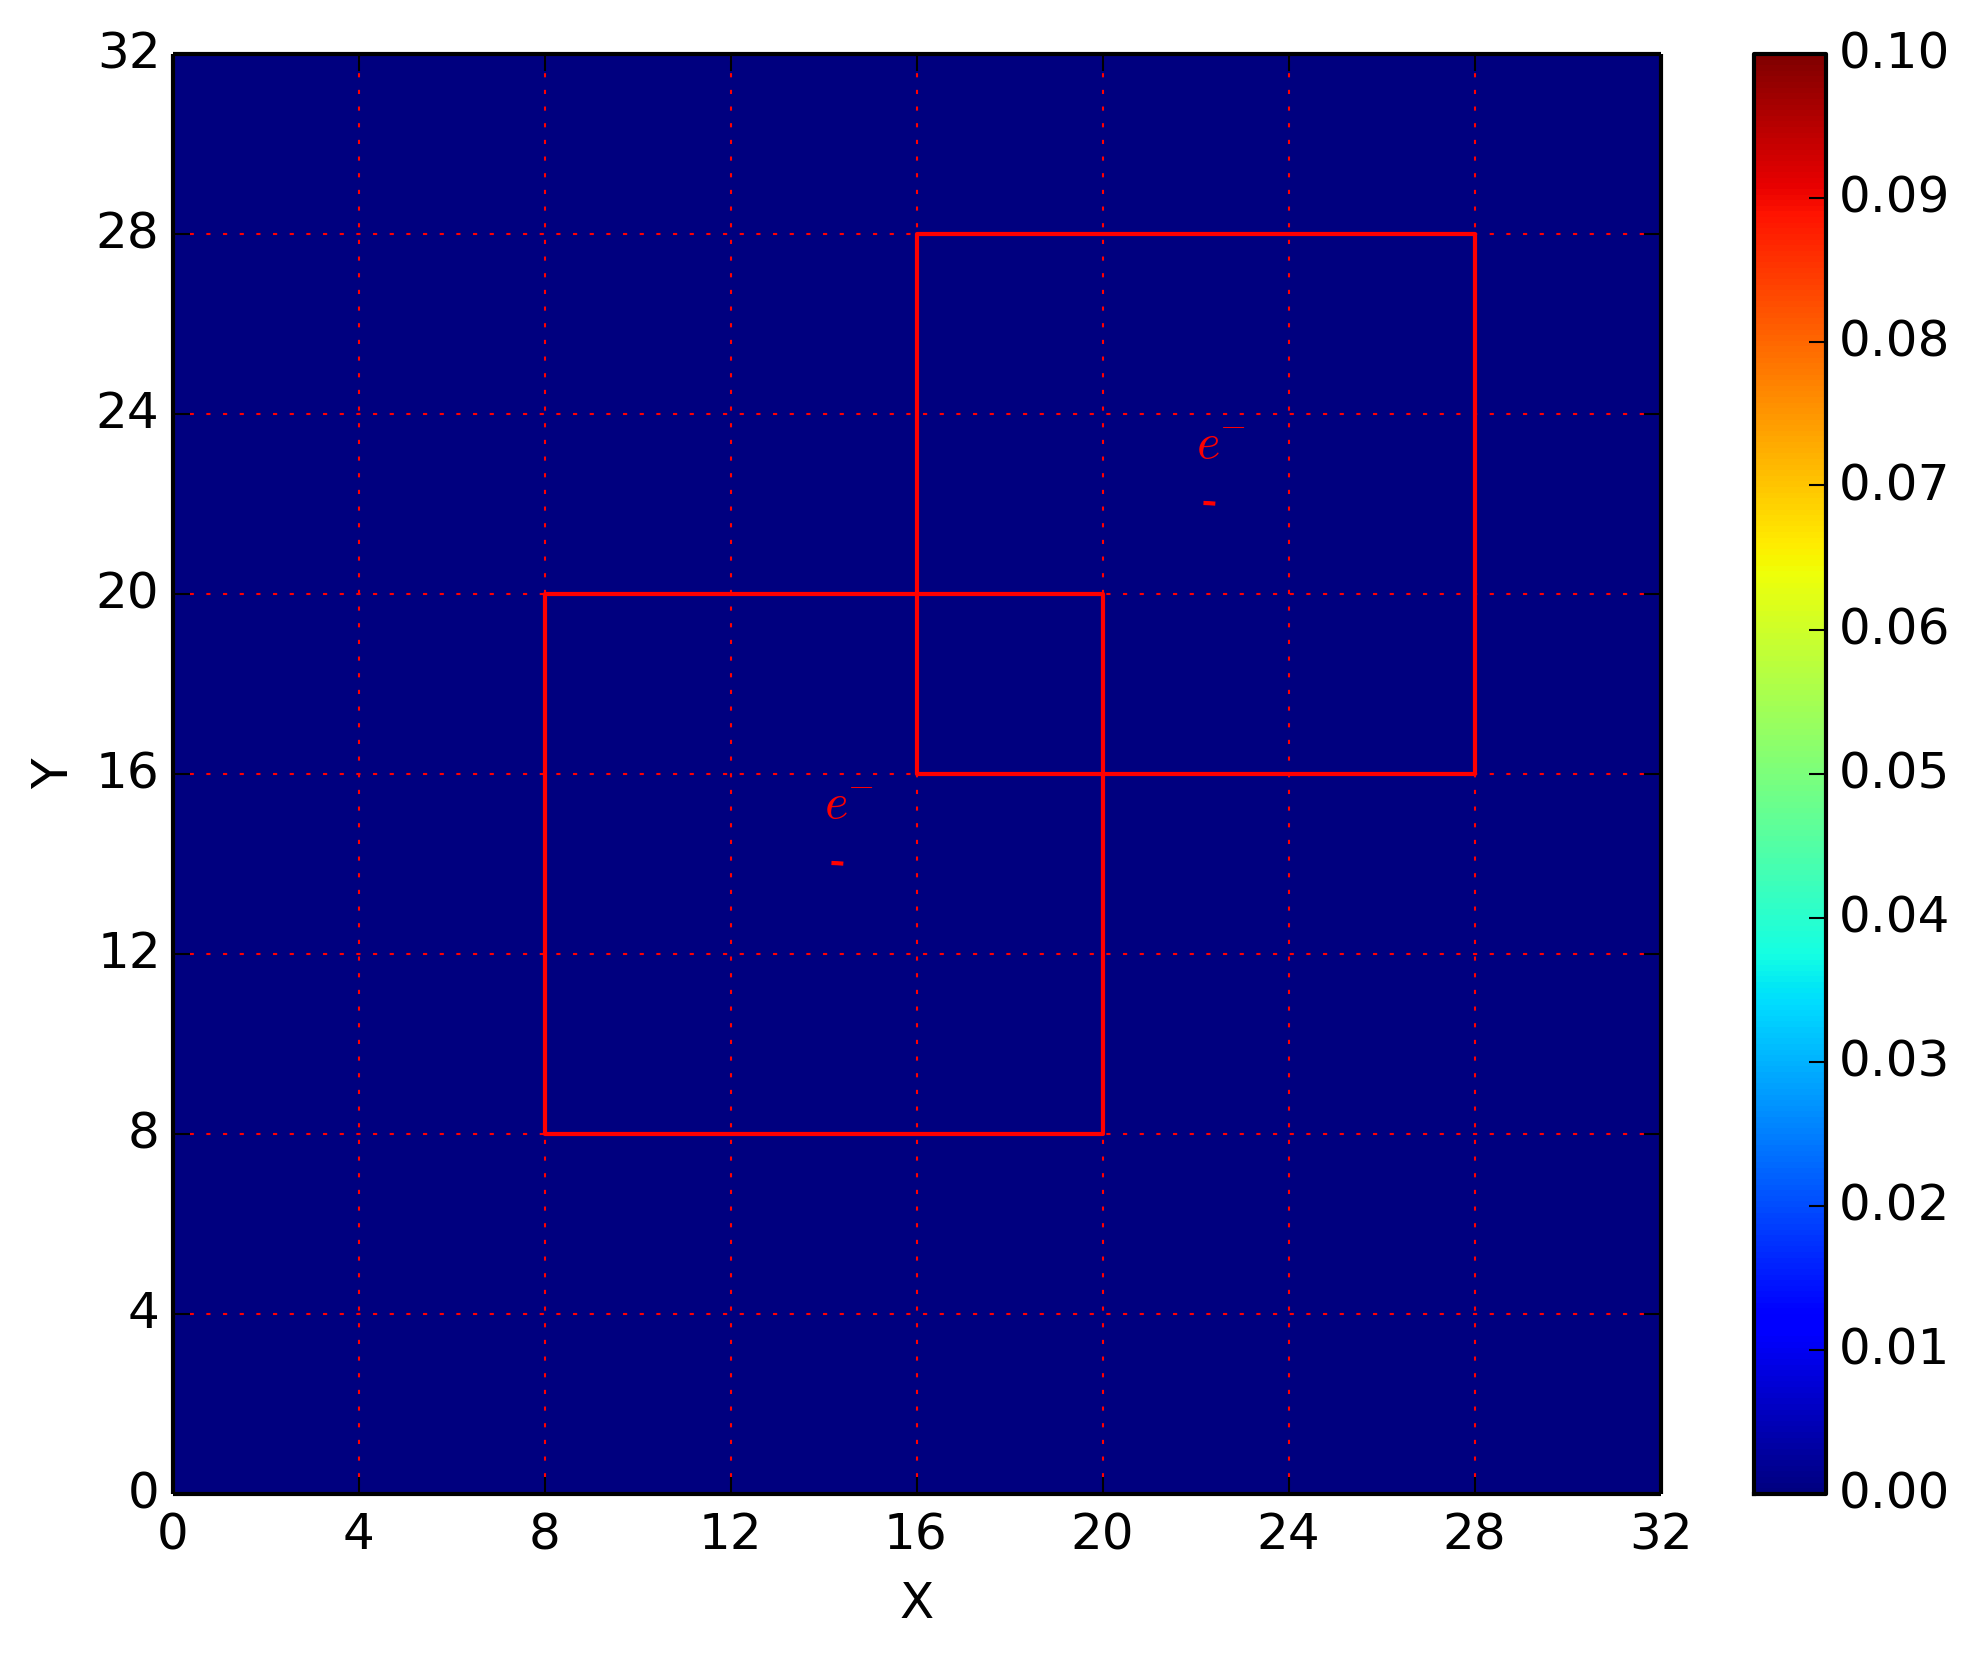
\includegraphics[width=0.49\textwidth]{Pictures/nearFieldTwoParticles.png}}
\caption[Nearfields of one and two particles]{Nearfields of one (a) and two (b) particles. The box at $(18,18)$ belongs to the Nearfield of both particles, marked with $e^{-}$. Notice the staggered red grid in the background. In this example we used 8 boxes, with 20 grid points each, and a spacing of 0.2 for each dimension. The plotted plane was chosen accordingly to the z - coordinate of the particle.}	
\label{fig: nearFields}
\end{figure}
%Bild des simulationsbereichs mit boxen. Wie werden boxen gez�hlt. 
%Bild 3D Box anhand dessen die einzelnen Schritte deutlich werden. 
% - push inside boxes
%1. set values on borders
% adjust values on borders
% push values on borders

\section{Particle Push and Nearfield Update}
\section{Particle History}
\section{Farfield Setup Before Simulation}
\section{Electron Scattering in an electromagnetic wave}
%======================== UPML ============================
%===========================================================
\chapter{Uniaxial Perfectly Matched Layer}

\part{Summary}
\part{Appendix}
\appendix
\chapter{Gauge Transformations}
\label{appendix: Gauge Transformations}
\noindent
In this chapter we want to show, that the gauge fields leave both the electric and magnetic fields and the corresponding potential equations invariant.
\section{Invariance of Fields}
We want to show that $\vec{E}' = \vec{E}$ and $\vec{B}' = \vec{B}$.
\beq
\bal
\vec{E}' &= -\vec{\nabla} \varphi' - \frac{\del \vec{A}'}{\del t} \nn \\
&= -\vec{\nabla} \left( \varphi - \frac{\del \psi}{\del t}\right) - \frac{\del}{\del t}\left( \vec{A} + \vec{\nabla} \psi\right) \nn \\
&= -\vec{\nabla}\varphi + \vec{\nabla}\left(\frac{\del \psi}{\del t}\right) -  \frac{\del \vec{A}}{\del t} - \frac{\del}{\del t} (\vec{\nabla} \psi) \nn\\
&= \vec{E}
\eal
\eeq
and
\beq
\bal
\vec{B}' &= \vec{\nabla} \times \vec{A}' \nn\\
&= \vec{\nabla} \times \left( \vec{A} + \vec{\nabla} \psi\right)\nn\\
&= \vec{\nabla}\times \vec{A} + \vec{\nabla}\times (\vec{\nabla} \psi)\nn\\
&= \vec{B}.
\eal
\eeq
\section{Invariance of Potential Equations}
Now we want to show the invariance of the potential equations. Therefore consider
\beq
\bal
-\Delta \varphi' - \vec{\nabla}\left(\frac{\del \vec{A}'}{\del t}\right) &= \frac{\rho}{\epsilon_0} \nn\\
\Longleftrightarrow -\Delta \left(\varphi - \frac{\del \psi}{\del t} \right) - \vec{\nabla}\left[ \frac{\del}{\del t} \left(\vec{A} + \vec{\nabla}\psi\right) \right] &=\frac{\rho}{\epsilon_0} \nn\\
\Longleftrightarrow -\Delta \varphi + \Delta\left(\frac{\del \psi}{\del t}\right) - \vec{\nabla}\left(\frac{\del \vec{A}}{\del t}\right) - \vec{\nabla}\left[ \frac{\del}{\del t}\left( \vec{\nabla}\psi\right) \right] &= \frac{\rho}{\epsilon_0} \nn\\
\Longleftrightarrow -\Delta \varphi - \vec{\nabla}\left(\frac{\del \vec{A}}{\del t}\right) &= \frac{\rho}{\epsilon_0} \nn\\
\eal
\eeq
and
\beq
\bal
\square \vec{A}' - \vec{\nabla} \left(\vec{\nabla} \vec{A}' + \frac{1}{c^2}\frac{\del \varphi' }{\del t} \right) &= -\mu_0\vec{j}\nn\\
\Longleftrightarrow \hat\square \left(\vec{A} + \vec{\nabla}\psi\right) - \vec{\nabla} \left[\vec{\nabla}  \left(\vec{A} + \vec{\nabla}\psi\right) + \frac{1}{c^2}\frac{\del}{\del t} \left(\varphi - \frac{\del \psi}{\del t} \right) \right] &= -\mu_0\vec{j}\nn\\
\Longleftrightarrow \hat\square \vec{A} + \square \left(\vec{\nabla}\psi\right) - \vec{\nabla} \left[\vec{\nabla} \vec{A} + \Delta \psi + \frac{1}{c^2}\frac{\del \varphi}{\del t} -  \frac{1}{c^2}\frac{\del^2 \psi}{\del t^2} \right] &= -\mu_0\vec{j}\nn\\
\Longleftrightarrow \hat\square \vec{A} + \square \left(\vec{\nabla}\psi\right) - \vec{\nabla} \left[\vec{\nabla} \vec{A} + \square \psi +  \frac{1}{c^2}\frac{\del \varphi}{\del t} \right] &= -\mu_0\vec{j}\nn\\
\Longleftrightarrow \hat\square \vec{A} - \vec{\nabla} \left(\vec{\nabla} \vec{A} + \frac{1}{c^2}\frac{\del \varphi}{\del t} \right) &= -\mu_0\vec{j}\nn\\
\eal
\eeq
\chapter{Retarded Potential Equations Fulfill Laurentz Gauge}
\label{appendix: Retarded Potential Equations Fulfill Laurentz Gauge}
\noindent
We show that the retarded potential equations 
\beq
\varphi(\vec{r},t) &=& \frac{1}{4\pi \epsilon_0} \int_{V} \frac{\rho(\vec{r}~', t_{ret})}{|\vec{r} - \vec{r}~'|} \dm \vec{r}~',\nn\\
\vec{A}(\vec{r},t) &=& \frac{\mu_0}{4\pi} \int_{V} \frac{\vec{j}(\vec{r}~', t_{ret})}{|\vec{r} - \vec{r}~'|} \dm \vec{r}~'\nn
\eeq
with $t_{ret} \coloneqq t - \frac{|\vec{r} - \vec{r}~'|}{c}$ fulfill the Laurentz Gauge
\beq
\vec{\nabla} \vec{A} + \frac{1}{c^2}\frac{\del \varphi}{\del t} = 0.\nn
\eeq
Plugging in yields
\beq
\label{eqn: step1}
\bal
\vec{\nabla} \vec{A} + \frac{1}{c^2}\frac{\del \varphi}{\del t} &= \frac{\mu_0}{4\pi} \int_{V} \vec{\nabla}_{\vec{r}}~ \frac{\vec{j}(\vec{r}~', t_{ret})}{|\vec{r} - \vec{r}~'|} \dm \vec{r}~' + \frac{1}{c^2}  \frac{1}{4\pi \epsilon_0} \int_{V} \frac{\del}{\del t}\frac{\rho(\vec{r}~', t_{ret})}{|\vec{r} - \vec{r}~'|} \dm \vec{r}~'\nn\\
&=  \frac{\mu_0}{4\pi} \int_{V} \vec{\nabla}_{\vec{r}}~ \frac{\vec{j}(\vec{r}~', t_{ret})}{|\vec{r} - \vec{r}~'|} \frac{\del}{\del t}\frac{\rho(\vec{r}~', t_{ret})}{|\vec{r} - \vec{r}~'|} \dm \vec{r}~',\nn\\
\eal
\eeq
where we used $c^2 = \frac{1}{\mu_0\epsilon_0}$. Now consider the first term in the integrand
\beq
\bal
\vec{\nabla}_{\vec{r}}~ \frac{\vec{j}(\vec{r}~', t_{ret})}{|\vec{r} - \vec{r}~'|} &= \vec{j}(\vec{r}~', t_{ret}) \vec{\nabla}_{\vec{r}} \left( \frac{1}{|\vec{r} - \vec{r}~'|}\right) + \frac{1}{|\vec{r} - \vec{r}~'|} \del_{t_{ret}}\vec{j}(\vec{r}~', t_{ret}) \vec{\nabla}_{\vec{r}}~ t_{ret}\nn \\
&= -\vec{j}(\vec{r}~', t_{ret}) \frac{\vec{r} - \vec{r}~'}{|\vec{r} - \vec{r}~'|^3} - \frac{1}{c} \frac{\vec{r} - \vec{r}~'}{|\vec{r} - \vec{r}~'|^2} \del_{t_{ret}}\vec{j}(\vec{r}~', t_{ret})
\eal
\eeq
On the other hand we also have
\beq
\bal
\vec{\nabla}_{\vec{r}~'}~ \frac{\vec{j}(\vec{r}~', t_{ret})}{|\vec{r} - \vec{r}~'|} &= \vec{j}(\vec{r}~', t_{ret}) \vec{\nabla}_{\vec{r}~'} \left( \frac{1}{|\vec{r} - \vec{r}~'|}\right) + \frac{1}{|\vec{r} - \vec{r}~'|} \left( \vec{\nabla}_{\vec{r}~'} \vec{j}(\vec{r}~', t_{ret})\Bigr |_{t_{ret}} + \del_{t_{ret}}\vec{j}(\vec{r}~', t_{ret}) \vec{\nabla}_{\vec{r}~'}~ t_{ret}\right)\nn \\
&= \vec{j}(\vec{r}~', t_{ret}) \frac{\vec{r} - \vec{r}~'}{|\vec{r} - \vec{r}~'|^3} + \frac{1}{|\vec{r} - \vec{r}~'|} \left( \vec{\nabla}_{\vec{r}~'} \vec{j}(\vec{r}~', t_{ret}) \Bigr |_{t_{ret}}+ \frac{1}{c}  \frac{\vec{r} - \vec{r}~'}{|\vec{r} - \vec{r}~'|} \del_{t_{ret}}\vec{j}(\vec{r}~', t_{ret}) \right),
\eal
\eeq
which means that we can write
\beq
\vec{\nabla}_{\vec{r}}~ \frac{\vec{j}(\vec{r}~', t_{ret})}{|\vec{r} - \vec{r}~'|} + \vec{\nabla}_{\vec{r}~'}~ \frac{\vec{j}(\vec{r}~', t_{ret})}{|\vec{r} - \vec{r}~'|} =  \frac{\vec{\nabla}_{\vec{r}~'} \vec{j}(\vec{r}~', t_{ret})\Bigr |_{t_{ret}}}{|\vec{r} - \vec{r}~'|}. \nn
\eeq
Plugging in this into \eqref{eqn: step1} yields
\beq
\vec{\nabla} \vec{A} + \frac{1}{c^2}\frac{\del \varphi}{\del t} = \frac{\mu_0}{4\pi} \int_{V} - \vec{\nabla}_{\vec{r}~'}~ \frac{\vec{j}(\vec{r}~', t_{ret})}{|\vec{r} - \vec{r}~'|} + \underbrace{ \frac{\vec{\nabla}_{\vec{r}~'} \vec{j}(\vec{r}~', t_{ret})\Bigr |_{t_{ret}}}{|\vec{r} - \vec{r}~'|} + \frac{\del}{\del t}\frac{\rho(\vec{r}~', t_{ret})}{|\vec{r} - \vec{r}~'|}}_{= 0 \text{ due to continuity equation}} ~\dm \vec{r}~'. \nn 
\eeq
For the remaining first term we use \textit{Stokes Law}
\beq
\vec{\nabla} \vec{A} + \frac{1}{c^2}\frac{\del \varphi}{\del t} = -\frac{\mu_0}{4\pi} \int_{V} \vec{\nabla}_{\vec{r}~'}~ \frac{\vec{j}(\vec{r}~', t_{ret})}{|\vec{r} - \vec{r}~'|} \dm \vec{r}~' =  - \frac{\mu_0}{4\pi} \oint_{\del V}  \frac{\vec{j}(\vec{r}~', t_{ret})}{|\vec{r} - \vec{r}~'|} \dm \vec{\sigma} = 0, \nn
\eeq
because the current density vanishes at infinity. That's what we wanted to show.
\chapter{Softwarestack}
\chapter{Code Documentation}
\chapter{Normalization}
%============================= Abbildungsverzeichnis ===========================
\listoffigures

%======================== Literaturverzeichnis ========================

\bibliography{reference}{}
\bibliographystyle{plain}

%================================= ERKL�RUNG=============================
\chapter*{Declaration}
\addcontentsline{toc}{chapter}{Declaration}
\vspace{1cm}
\noindent
Erkl�rung:\\
\newline
Hiermit erkl�re ich, die vorliegende Arbeit selbst�ndig verfasst zu haben und keine anderen als die in der Arbeit angegebenen Quellen und Hilfsmittel benutzt zu haben.\\
\newline
M�nchen, 17.07.2017 \\
\vspace{2cm}
\\
\line(1,0){300}\\
David Symhoven



\end{document}











